\documentclass[1p]{elsarticle_modified}
%\bibliographystyle{elsarticle-num}

%\usepackage[colorlinks]{hyperref}
%\usepackage{abbrmath_seonhwa} %\Abb, \Ascr, \Acal ,\Abf, \Afrak
\usepackage{amsfonts}
\usepackage{amssymb}
\usepackage{amsmath}
\usepackage{amsthm}
\usepackage{scalefnt}
\usepackage{amsbsy}
\usepackage{kotex}
\usepackage{caption}
\usepackage{subfig}
\usepackage{color}
\usepackage{graphicx}
\usepackage{xcolor} %% white, black, red, green, blue, cyan, magenta, yellow
\usepackage{float}
\usepackage{setspace}
\usepackage{hyperref}

\usepackage{tikz}
\usetikzlibrary{arrows}

\usepackage{multirow}
\usepackage{array} % fixed length table
\usepackage{hhline}

%%%%%%%%%%%%%%%%%%%%%
\makeatletter
\renewcommand*\env@matrix[1][\arraystretch]{%
	\edef\arraystretch{#1}%
	\hskip -\arraycolsep
	\let\@ifnextchar\new@ifnextchar
	\array{*\c@MaxMatrixCols c}}
\makeatother %https://tex.stackexchange.com/questions/14071/how-can-i-increase-the-line-spacing-in-a-matrix
%%%%%%%%%%%%%%%

\usepackage[normalem]{ulem}

\newcommand{\msout}[1]{\ifmmode\text{\sout{\ensuremath{#1}}}\else\sout{#1}\fi}
%SOURCE: \msout is \stkout macro in https://tex.stackexchange.com/questions/20609/strikeout-in-math-mode

\newcommand{\cancel}[1]{
	\ifmmode
	{\color{red}\msout{#1}}
	\else
	{\color{red}\sout{#1}}
	\fi
}

\newcommand{\add}[1]{
	{\color{blue}\uwave{#1}}
}

\newcommand{\replace}[2]{
	\ifmmode
	{\color{red}\msout{#1}}{\color{blue}\uwave{#2}}
	\else
	{\color{red}\sout{#1}}{\color{blue}\uwave{#2}}
	\fi
}

\newcommand{\Sol}{\mathcal{S}} %segment
\newcommand{\D}{D} %diagram
\newcommand{\A}{\mathcal{A}} %arc


%%%%%%%%%%%%%%%%%%%%%%%%%%%%%5 test

\def\sl{\operatorname{\textup{SL}}(2,\Cbb)}
\def\psl{\operatorname{\textup{PSL}}(2,\Cbb)}
\def\quan{\mkern 1mu \triangleright \mkern 1mu}

\theoremstyle{definition}
\newtheorem{thm}{Theorem}[section]
\newtheorem{prop}[thm]{Proposition}
\newtheorem{lem}[thm]{Lemma}
\newtheorem{ques}[thm]{Question}
\newtheorem{cor}[thm]{Corollary}
\newtheorem{defn}[thm]{Definition}
\newtheorem{exam}[thm]{Example}
\newtheorem{rmk}[thm]{Remark}
\newtheorem{alg}[thm]{Algorithm}

\newcommand{\I}{\sqrt{-1}}
\begin{document}

%\begin{frontmatter}
%
%\title{Boundary parabolic representations of knots up to 8 crossings}
%
%%% Group authors per affiliation:
%\author{Yunhi Cho} 
%\address{Department of Mathematics, University of Seoul, Seoul, Korea}
%\ead{yhcho@uos.ac.kr}
%
%
%\author{Seonhwa Kim} %\fnref{s_kim}}
%\address{Center for Geometry and Physics, Institute for Basic Science, Pohang, 37673, Korea}
%\ead{ryeona17@ibs.re.kr}
%
%\author{Hyuk Kim}
%\address{Department of Mathematical Sciences, Seoul National University, Seoul 08826, Korea}
%\ead{hyukkim@snu.ac.kr}
%
%\author{Seokbeom Yoon}
%\address{Department of Mathematical Sciences, Seoul National University, Seoul, 08826,  Korea}
%\ead{sbyoon15@snu.ac.kr}
%
%\begin{abstract}
%We find all boundary parabolic representation of knots up to 8 crossings.
%
%\end{abstract}
%\begin{keyword}
%    \MSC[2010] 57M25 
%\end{keyword}
%
%\end{frontmatter}

%\linenumbers
%\tableofcontents
%
\newcommand\colored[1]{\textcolor{white}{\rule[-0.35ex]{0.8em}{1.4ex}}\kern-0.8em\color{red} #1}%
%\newcommand\colored[1]{\textcolor{white}{ #1}\kern-2.17ex	\textcolor{white}{ #1}\kern-1.81ex	\textcolor{white}{ #1}\kern-2.15ex\color{red}#1	}

{\Large $\underline{12a_{0874}~(K12a_{0874})}$}

\setlength{\tabcolsep}{10pt}
\renewcommand{\arraystretch}{1.6}
\vspace{1cm}\begin{tabular}{m{100pt}>{\centering\arraybackslash}m{274pt}}
\multirow{5}{120pt}{
	\centering
	\includegraphics[width=112pt]{../../../GIT/diagram.site/Diagrams/png/1675_12a_0874.png}\\
\ \ \ A knot diagram\footnotemark}&
\allowdisplaybreaks
\textbf{Linearized knot diagam} \\
\cline{2-2}
 &
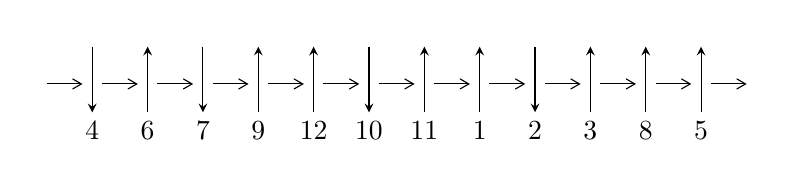
\begin{tikzpicture}[x=20pt, y=17pt]
	% nodes
	\node (C0) at (0, 0) {};
	\node (C1) at (1, 0) {};
	\node (C1U) at (1, +1) {};
	\node (C1D) at (1, -1) {4};

	\node (C2) at (2, 0) {};
	\node (C2U) at (2, +1) {};
	\node (C2D) at (2, -1) {6};

	\node (C3) at (3, 0) {};
	\node (C3U) at (3, +1) {};
	\node (C3D) at (3, -1) {7};

	\node (C4) at (4, 0) {};
	\node (C4U) at (4, +1) {};
	\node (C4D) at (4, -1) {9};

	\node (C5) at (5, 0) {};
	\node (C5U) at (5, +1) {};
	\node (C5D) at (5, -1) {12};

	\node (C6) at (6, 0) {};
	\node (C6U) at (6, +1) {};
	\node (C6D) at (6, -1) {10};

	\node (C7) at (7, 0) {};
	\node (C7U) at (7, +1) {};
	\node (C7D) at (7, -1) {11};

	\node (C8) at (8, 0) {};
	\node (C8U) at (8, +1) {};
	\node (C8D) at (8, -1) {1};

	\node (C9) at (9, 0) {};
	\node (C9U) at (9, +1) {};
	\node (C9D) at (9, -1) {2};

	\node (C10) at (10, 0) {};
	\node (C10U) at (10, +1) {};
	\node (C10D) at (10, -1) {3};

	\node (C11) at (11, 0) {};
	\node (C11U) at (11, +1) {};
	\node (C11D) at (11, -1) {8};

	\node (C12) at (12, 0) {};
	\node (C12U) at (12, +1) {};
	\node (C12D) at (12, -1) {5};
	\node (C13) at (13, 0) {};

	% arrows
	\draw[->,>={angle 60}]
	(C0) edge (C1) (C1) edge (C2) (C2) edge (C3) (C3) edge (C4) (C4) edge (C5) (C5) edge (C6) (C6) edge (C7) (C7) edge (C8) (C8) edge (C9) (C9) edge (C10) (C10) edge (C11) (C11) edge (C12) (C12) edge (C13) ;	\draw[->,>=stealth]
	(C1U) edge (C1D) (C2D) edge (C2U) (C3U) edge (C3D) (C4D) edge (C4U) (C5D) edge (C5U) (C6U) edge (C6D) (C7D) edge (C7U) (C8D) edge (C8U) (C9U) edge (C9D) (C10D) edge (C10U) (C11D) edge (C11U) (C12D) edge (C12U) ;
	\end{tikzpicture} \\
\hhline{~~} \\& 
\textbf{Solving Sequence} \\ \cline{2-2} 
 &
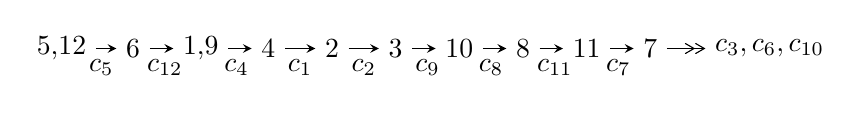
\begin{tikzpicture}[x=23pt, y=7pt]
	% node
	\node (A0) at (-1/8, 0) {5,12};
	\node (A1) at (1, 0) {6};
	\node (A2) at (33/16, 0) {1,9};
	\node (A3) at (25/8, 0) {4};
	\node (A4) at (33/8, 0) {2};
	\node (A5) at (41/8, 0) {3};
	\node (A6) at (49/8, 0) {10};
	\node (A7) at (57/8, 0) {8};
	\node (A8) at (65/8, 0) {11};
	\node (A9) at (73/8, 0) {7};
	\node (C1) at (1/2, -1) {$c_{5}$};
	\node (C2) at (3/2, -1) {$c_{12}$};
	\node (C3) at (21/8, -1) {$c_{4}$};
	\node (C4) at (29/8, -1) {$c_{1}$};
	\node (C5) at (37/8, -1) {$c_{2}$};
	\node (C6) at (45/8, -1) {$c_{9}$};
	\node (C7) at (53/8, -1) {$c_{8}$};
	\node (C8) at (61/8, -1) {$c_{11}$};
	\node (C9) at (69/8, -1) {$c_{7}$};
	\node (A10) at (11, 0) {$c_{3},c_{6},c_{10}$};

	% edge
	\draw[->,>=stealth]	
	(A0) edge (A1) (A1) edge (A2) (A2) edge (A3) (A3) edge (A4) (A4) edge (A5) (A5) edge (A6) (A6) edge (A7) (A7) edge (A8) (A8) edge (A9) ;
	\draw[->>,>={angle 60}]	
	(A9) edge (A10);
\end{tikzpicture} \\ 

\end{tabular} \\

\footnotetext{
The image of knot diagram is generated by the software ``\textbf{Draw programme}" developed by Andrew Bartholomew(\url{http://www.layer8.co.uk/maths/draw/index.htm\#Running-draw}), where we modified some parts for our purpose(\url{https://github.com/CATsTAILs/LinksPainter}).
}\phantom \\ \newline 
\centering \textbf{Ideals for irreducible components\footnotemark of $X_{\text{par}}$} 
 
\begin{align*}
I^u_{1}&=\langle 
-1.84886\times10^{1402} u^{190}+3.70297\times10^{1402} u^{189}+\cdots+1.63068\times10^{1404} b+1.52642\times10^{1408},\\
\phantom{I^u_{1}}&\phantom{= \langle  }-2.20329\times10^{1408} u^{190}+6.86665\times10^{1407} u^{189}+\cdots+4.27740\times10^{1409} a+4.99679\times10^{1413},\\
\phantom{I^u_{1}}&\phantom{= \langle  }u^{191}+65 u^{189}+\cdots-7345527 u+262307\rangle \\
I^u_{2}&=\langle 
2.77823\times10^{73} u^{49}+1.70736\times10^{73} u^{48}+\cdots+7.28128\times10^{73} b-2.44122\times10^{74},\\
\phantom{I^u_{2}}&\phantom{= \langle  }1.03235\times10^{75} u^{49}+1.05630\times10^{75} u^{48}+\cdots+7.28128\times10^{73} a+2.83270\times10^{75},\;u^{50}+u^{49}+\cdots+2 u+1\rangle \\
\\
\end{align*}
\raggedright * 2 irreducible components of $\dim_{\mathbb{C}}=0$, with total 241 representations.\\
\footnotetext{All coefficients of polynomials are rational numbers. But the coefficients are sometimes approximated in decimal forms when there is not enough margin.}
\newpage
\renewcommand{\arraystretch}{1}
\centering \section*{I. $I^u_{1}= \langle -1.85\times10^{1402} u^{190}+3.70\times10^{1402} u^{189}+\cdots+1.63\times10^{1404} b+1.53\times10^{1408},\;-2.20\times10^{1408} u^{190}+6.87\times10^{1407} u^{189}+\cdots+4.28\times10^{1409} a+5.00\times10^{1413},\;u^{191}+65 u^{189}+\cdots-7345527 u+262307 \rangle$}
\flushleft \textbf{(i) Arc colorings}\\
\begin{tabular}{m{7pt} m{180pt} m{7pt} m{180pt} }
\flushright $a_{5}=$&$\begin{pmatrix}1\\0\end{pmatrix}$ \\
\flushright $a_{12}=$&$\begin{pmatrix}0\\u\end{pmatrix}$ \\
\flushright $a_{6}=$&$\begin{pmatrix}1\\- u^2\end{pmatrix}$ \\
\flushright $a_{1}=$&$\begin{pmatrix}u\\u\end{pmatrix}$ \\
\flushright $a_{9}=$&$\begin{pmatrix}0.0515100 u^{190}-0.0160533 u^{189}+\cdots+326321. u-11681.9\\0.0113379 u^{190}-0.0227081 u^{189}+\cdots+258745. u-9360.63\end{pmatrix}$ \\
\flushright $a_{4}=$&$\begin{pmatrix}0.0586402 u^{190}+0.144311 u^{189}+\cdots-1.14998\times10^{6} u+42130.4\\0.0514121 u^{190}+0.0955835 u^{189}+\cdots-729887. u+26842.3\end{pmatrix}$ \\
\flushright $a_{2}=$&$\begin{pmatrix}0.0935137 u^{190}+0.0724429 u^{189}+\cdots-477887. u+18316.9\\0.0288888 u^{190}+0.0540440 u^{189}+\cdots-432033. u+15860.7\end{pmatrix}$ \\
\flushright $a_{3}=$&$\begin{pmatrix}0.0640409 u^{190}+0.0599123 u^{189}+\cdots-402318. u+15175.3\\0.00513012 u^{190}+0.0403217 u^{189}+\cdots-347720. u+12573.8\end{pmatrix}$ \\
\flushright $a_{10}=$&$\begin{pmatrix}-0.0724069 u^{190}-0.0906965 u^{189}+\cdots+611737. u-23521.2\\-0.0645735 u^{190}-0.0493419 u^{189}+\cdots+237286. u-9472.89\end{pmatrix}$ \\
\flushright $a_{8}=$&$\begin{pmatrix}0.0235649 u^{190}-0.0269071 u^{189}+\cdots+364666. u-13427.4\\-0.0166072 u^{190}-0.0335619 u^{189}+\cdots+297090. u-11106.2\end{pmatrix}$ \\
\flushright $a_{11}=$&$\begin{pmatrix}-0.117562 u^{190}+0.0353139 u^{189}+\cdots-638817. u+21444.7\\-0.0523487 u^{190}+0.0300864 u^{189}+\cdots-450943. u+15665.9\end{pmatrix}$ \\
\flushright $a_{7}=$&$\begin{pmatrix}-0.161698 u^{190}-0.0975729 u^{189}+\cdots+566662. u-23287.5\\-0.107800 u^{190}-0.0856358 u^{189}+\cdots+547467. u-21437.9\end{pmatrix}$\\&\end{tabular}
\flushleft \textbf{(ii) Obstruction class $= -1$}\\~\\
\flushleft \textbf{(iii) Cusp Shapes $= 0.0664855 u^{190}+0.106706 u^{189}+\cdots-806183. u+28495.4$}\\~\\
\newpage\renewcommand{\arraystretch}{1}
\flushleft \textbf{(iv) u-Polynomials at the component}\newline \\
\begin{tabular}{m{50pt}|m{274pt}}
Crossings & \hspace{64pt}u-Polynomials at each crossing \\
\hline $$\begin{aligned}c_{1}\end{aligned}$$&$\begin{aligned}
&u^{191}+8 u^{190}+\cdots+12090 u-521
\end{aligned}$\\
\hline $$\begin{aligned}c_{2}\end{aligned}$$&$\begin{aligned}
&u^{191}+9 u^{189}+\cdots+26856 u-3123
\end{aligned}$\\
\hline $$\begin{aligned}c_{3}\end{aligned}$$&$\begin{aligned}
&u^{191}+8 u^{190}+\cdots-40446 u-4563
\end{aligned}$\\
\hline $$\begin{aligned}c_{4}\end{aligned}$$&$\begin{aligned}
&u^{191}+23 u^{189}+\cdots-6088215 u-1128983
\end{aligned}$\\
\hline $$\begin{aligned}c_{5},c_{12}\end{aligned}$$&$\begin{aligned}
&u^{191}+65 u^{189}+\cdots-7345527 u-262307
\end{aligned}$\\
\hline $$\begin{aligned}c_{6}\end{aligned}$$&$\begin{aligned}
&u^{191}+2 u^{190}+\cdots-26 u-1
\end{aligned}$\\
\hline $$\begin{aligned}c_{7},c_{11}\end{aligned}$$&$\begin{aligned}
&u^{191}-4 u^{190}+\cdots-644237242 u-33057935
\end{aligned}$\\
\hline $$\begin{aligned}c_{8}\end{aligned}$$&$\begin{aligned}
&u^{191}+4 u^{190}+\cdots-14 u-1
\end{aligned}$\\
\hline $$\begin{aligned}c_{9}\end{aligned}$$&$\begin{aligned}
&u^{191}+3 u^{190}+\cdots+2081393442 u-208449613
\end{aligned}$\\
\hline $$\begin{aligned}c_{10}\end{aligned}$$&$\begin{aligned}
&u^{191}+4 u^{190}+\cdots-517308 u-92933
\end{aligned}$\\
\hline
\end{tabular}\\~\\
\newpage\renewcommand{\arraystretch}{1}
\flushleft \textbf{(v) Riley Polynomials at the component}\newline \\
\begin{tabular}{m{50pt}|m{274pt}}
Crossings & \hspace{64pt}Riley Polynomials at each crossing \\
\hline $$\begin{aligned}c_{1}\end{aligned}$$&$\begin{aligned}
&y^{191}+18 y^{190}+\cdots+7672754 y-271441
\end{aligned}$\\
\hline $$\begin{aligned}c_{2}\end{aligned}$$&$\begin{aligned}
&y^{191}+18 y^{190}+\cdots-1093867848 y-9753129
\end{aligned}$\\
\hline $$\begin{aligned}c_{3}\end{aligned}$$&$\begin{aligned}
&y^{191}+48 y^{190}+\cdots-547954632 y-20820969
\end{aligned}$\\
\hline $$\begin{aligned}c_{4}\end{aligned}$$&$\begin{aligned}
&y^{191}+46 y^{190}+\cdots-71896540462205 y-1274602614289
\end{aligned}$\\
\hline $$\begin{aligned}c_{5},c_{12}\end{aligned}$$&$\begin{aligned}
&y^{191}+130 y^{190}+\cdots+5931925730613 y-68804962249
\end{aligned}$\\
\hline $$\begin{aligned}c_{6}\end{aligned}$$&$\begin{aligned}
&y^{191}-14 y^{190}+\cdots+150 y-1
\end{aligned}$\\
\hline $$\begin{aligned}c_{7},c_{11}\end{aligned}$$&$\begin{aligned}
&y^{191}-140 y^{190}+\cdots+148730603959730924 y-1092827066464225
\end{aligned}$\\
\hline $$\begin{aligned}c_{8}\end{aligned}$$&$\begin{aligned}
&y^{191}+16 y^{190}+\cdots-1830 y-1
\end{aligned}$\\
\hline $$\begin{aligned}c_{9}\end{aligned}$$&$\begin{aligned}
&y^{191}-55 y^{190}+\cdots+2565423313669011206 y-43451241159849769
\end{aligned}$\\
\hline $$\begin{aligned}c_{10}\end{aligned}$$&$\begin{aligned}
&y^{191}-24 y^{190}+\cdots+682916036430 y-8636542489
\end{aligned}$\\
\hline
\end{tabular}\\~\\
\newpage\flushleft \textbf{(vi) Complex Volumes and Cusp Shapes}
$$\begin{array}{c|c|c}  
\text{Solutions to }I^u_{1}& \I (\text{vol} + \sqrt{-1}CS) & \text{Cusp shape}\\
 \hline 
\begin{aligned}
u &= \phantom{-}0.512846 + 0.859954 I \\
a &= -0.993688 + 0.949455 I \\
b &= -0.962967 + 0.962306 I\end{aligned}
 & \phantom{-}1.62279 - 0.11399 I & \phantom{-0.000000 } 0 \\ \hline\begin{aligned}
u &= \phantom{-}0.512846 - 0.859954 I \\
a &= -0.993688 - 0.949455 I \\
b &= -0.962967 - 0.962306 I\end{aligned}
 & \phantom{-}1.62279 + 0.11399 I & \phantom{-0.000000 } 0 \\ \hline\begin{aligned}
u &= \phantom{-}0.978114 + 0.183462 I \\
a &= -0.473054 + 0.830311 I \\
b &= \phantom{-}0.619112 + 1.108490 I\end{aligned}
 & \phantom{-}3.58690 + 5.22077 I & \phantom{-0.000000 } 0 \\ \hline\begin{aligned}
u &= \phantom{-}0.978114 - 0.183462 I \\
a &= -0.473054 - 0.830311 I \\
b &= \phantom{-}0.619112 - 1.108490 I\end{aligned}
 & \phantom{-}3.58690 - 5.22077 I & \phantom{-0.000000 } 0 \\ \hline\begin{aligned}
u &= -0.102811 + 1.007920 I \\
a &= -3.34076 - 0.79703 I \\
b &= \phantom{-}0.387767 + 0.166638 I\end{aligned}
 & -1.76777 - 0.26711 I & \phantom{-0.000000 } 0 \\ \hline\begin{aligned}
u &= -0.102811 - 1.007920 I \\
a &= -3.34076 + 0.79703 I \\
b &= \phantom{-}0.387767 - 0.166638 I\end{aligned}
 & -1.76777 + 0.26711 I & \phantom{-0.000000 } 0 \\ \hline\begin{aligned}
u &= \phantom{-}0.652465 + 0.737354 I \\
a &= \phantom{-}0.11217 + 2.09971 I \\
b &= \phantom{-}0.66513 + 1.32327 I\end{aligned}
 & \phantom{-}4.43750 - 0.16046 I & \phantom{-0.000000 } 0 \\ \hline\begin{aligned}
u &= \phantom{-}0.652465 - 0.737354 I \\
a &= \phantom{-}0.11217 - 2.09971 I \\
b &= \phantom{-}0.66513 - 1.32327 I\end{aligned}
 & \phantom{-}4.43750 + 0.16046 I & \phantom{-0.000000 } 0 \\ \hline\begin{aligned}
u &= -0.063400 + 0.979157 I \\
a &= \phantom{-}1.66806 - 1.73143 I \\
b &= -0.255460 - 0.917578 I\end{aligned}
 & -3.41286 - 0.27827 I & \phantom{-0.000000 } 0 \\ \hline\begin{aligned}
u &= -0.063400 - 0.979157 I \\
a &= \phantom{-}1.66806 + 1.73143 I \\
b &= -0.255460 + 0.917578 I\end{aligned}
 & -3.41286 + 0.27827 I & \phantom{-0.000000 } 0\\
 \hline 
 \end{array}$$\newpage$$\begin{array}{c|c|c}  
\text{Solutions to }I^u_{1}& \I (\text{vol} + \sqrt{-1}CS) & \text{Cusp shape}\\
 \hline 
\begin{aligned}
u &= \phantom{-}0.334797 + 0.964987 I \\
a &= \phantom{-}0.360107 - 0.486954 I \\
b &= \phantom{-}0.727671 - 0.923644 I\end{aligned}
 & \phantom{-}4.04608 - 4.03130 I & \phantom{-0.000000 } 0 \\ \hline\begin{aligned}
u &= \phantom{-}0.334797 - 0.964987 I \\
a &= \phantom{-}0.360107 + 0.486954 I \\
b &= \phantom{-}0.727671 + 0.923644 I\end{aligned}
 & \phantom{-}4.04608 + 4.03130 I & \phantom{-0.000000 } 0 \\ \hline\begin{aligned}
u &= -0.245261 + 0.991590 I \\
a &= \phantom{-}1.08011 + 1.00475 I \\
b &= \phantom{-}1.22574 + 1.23155 I\end{aligned}
 & \phantom{-}3.24219 - 4.65971 I & \phantom{-0.000000 } 0 \\ \hline\begin{aligned}
u &= -0.245261 - 0.991590 I \\
a &= \phantom{-}1.08011 - 1.00475 I \\
b &= \phantom{-}1.22574 - 1.23155 I\end{aligned}
 & \phantom{-}3.24219 + 4.65971 I & \phantom{-0.000000 } 0 \\ \hline\begin{aligned}
u &= -0.923435 + 0.314359 I \\
a &= -0.093251 - 0.285405 I \\
b &= \phantom{-}0.862564 - 0.892525 I\end{aligned}
 & -0.56099 - 10.00740 I & \phantom{-0.000000 } 0 \\ \hline\begin{aligned}
u &= -0.923435 - 0.314359 I \\
a &= -0.093251 + 0.285405 I \\
b &= \phantom{-}0.862564 + 0.892525 I\end{aligned}
 & -0.56099 + 10.00740 I & \phantom{-0.000000 } 0 \\ \hline\begin{aligned}
u &= \phantom{-}0.067457 + 0.965865 I \\
a &= \phantom{-}0.324948 - 0.329435 I \\
b &= \phantom{-}0.745054 + 0.046203 I\end{aligned}
 & -1.96101 - 1.49328 I & \phantom{-0.000000 } 0 \\ \hline\begin{aligned}
u &= \phantom{-}0.067457 - 0.965865 I \\
a &= \phantom{-}0.324948 + 0.329435 I \\
b &= \phantom{-}0.745054 - 0.046203 I\end{aligned}
 & -1.96101 + 1.49328 I & \phantom{-0.000000 } 0 \\ \hline\begin{aligned}
u &= \phantom{-}0.763160 + 0.575586 I \\
a &= -0.02349 - 1.82947 I \\
b &= -0.900127 - 1.006580 I\end{aligned}
 & \phantom{-}4.29389 - 8.15564 I & \phantom{-0.000000 } 0 \\ \hline\begin{aligned}
u &= \phantom{-}0.763160 - 0.575586 I \\
a &= -0.02349 + 1.82947 I \\
b &= -0.900127 + 1.006580 I\end{aligned}
 & \phantom{-}4.29389 + 8.15564 I & \phantom{-0.000000 } 0\\
 \hline 
 \end{array}$$\newpage$$\begin{array}{c|c|c}  
\text{Solutions to }I^u_{1}& \I (\text{vol} + \sqrt{-1}CS) & \text{Cusp shape}\\
 \hline 
\begin{aligned}
u &= \phantom{-}0.351723 + 0.887873 I \\
a &= -0.176619 + 0.859935 I \\
b &= -0.802411 + 0.916053 I\end{aligned}
 & \phantom{-}3.14538 + 1.39324 I & \phantom{-0.000000 } 0 \\ \hline\begin{aligned}
u &= \phantom{-}0.351723 - 0.887873 I \\
a &= -0.176619 - 0.859935 I \\
b &= -0.802411 - 0.916053 I\end{aligned}
 & \phantom{-}3.14538 - 1.39324 I & \phantom{-0.000000 } 0 \\ \hline\begin{aligned}
u &= -0.420057 + 0.958849 I \\
a &= \phantom{-}0.961807 + 0.025499 I \\
b &= \phantom{-}1.38879 + 0.46497 I\end{aligned}
 & \phantom{-}0.86595 - 4.74204 I & \phantom{-0.000000 } 0 \\ \hline\begin{aligned}
u &= -0.420057 - 0.958849 I \\
a &= \phantom{-}0.961807 - 0.025499 I \\
b &= \phantom{-}1.38879 - 0.46497 I\end{aligned}
 & \phantom{-}0.86595 + 4.74204 I & \phantom{-0.000000 } 0 \\ \hline\begin{aligned}
u &= \phantom{-}0.196400 + 1.046200 I \\
a &= -1.57183 - 2.09208 I \\
b &= -0.046973 - 0.660831 I\end{aligned}
 & -0.23823 + 11.38630 I & \phantom{-0.000000 } 0 \\ \hline\begin{aligned}
u &= \phantom{-}0.196400 - 1.046200 I \\
a &= -1.57183 + 2.09208 I \\
b &= -0.046973 + 0.660831 I\end{aligned}
 & -0.23823 - 11.38630 I & \phantom{-0.000000 } 0 \\ \hline\begin{aligned}
u &= \phantom{-}1.053650 + 0.155311 I \\
a &= \phantom{-}0.007011 + 0.199597 I \\
b &= -0.767990 + 0.943186 I\end{aligned}
 & \phantom{-}2.09784 - 6.73290 I & \phantom{-0.000000 } 0 \\ \hline\begin{aligned}
u &= \phantom{-}1.053650 - 0.155311 I \\
a &= \phantom{-}0.007011 - 0.199597 I \\
b &= -0.767990 - 0.943186 I\end{aligned}
 & \phantom{-}2.09784 + 6.73290 I & \phantom{-0.000000 } 0 \\ \hline\begin{aligned}
u &= -0.636027 + 0.683004 I \\
a &= \phantom{-}0.423049 - 0.420854 I \\
b &= \phantom{-}0.670440 + 0.234980 I\end{aligned}
 & \phantom{-}1.89166 - 2.30214 I & \phantom{-0.000000 } 0 \\ \hline\begin{aligned}
u &= -0.636027 - 0.683004 I \\
a &= \phantom{-}0.423049 + 0.420854 I \\
b &= \phantom{-}0.670440 - 0.234980 I\end{aligned}
 & \phantom{-}1.89166 + 2.30214 I & \phantom{-0.000000 } 0\\
 \hline 
 \end{array}$$\newpage$$\begin{array}{c|c|c}  
\text{Solutions to }I^u_{1}& \I (\text{vol} + \sqrt{-1}CS) & \text{Cusp shape}\\
 \hline 
\begin{aligned}
u &= \phantom{-}0.203809 + 1.048740 I \\
a &= \phantom{-}1.19180 + 1.78538 I \\
b &= -0.145495 + 0.643514 I\end{aligned}
 & \phantom{-}0.87699 + 3.92374 I & \phantom{-0.000000 } 0 \\ \hline\begin{aligned}
u &= \phantom{-}0.203809 - 1.048740 I \\
a &= \phantom{-}1.19180 - 1.78538 I \\
b &= -0.145495 - 0.643514 I\end{aligned}
 & \phantom{-}0.87699 - 3.92374 I & \phantom{-0.000000 } 0 \\ \hline\begin{aligned}
u &= -0.149392 + 1.063000 I \\
a &= \phantom{-}1.03449 - 1.56066 I \\
b &= \phantom{-}0.068658 - 0.906663 I\end{aligned}
 & -1.78563 - 3.42046 I & \phantom{-0.000000 } 0 \\ \hline\begin{aligned}
u &= -0.149392 - 1.063000 I \\
a &= \phantom{-}1.03449 + 1.56066 I \\
b &= \phantom{-}0.068658 + 0.906663 I\end{aligned}
 & -1.78563 + 3.42046 I & \phantom{-0.000000 } 0 \\ \hline\begin{aligned}
u &= -0.125292 + 0.912031 I \\
a &= -1.01216 + 3.00472 I \\
b &= -0.208639 + 0.568525 I\end{aligned}
 & -0.797459 - 0.334339 I & \phantom{-0.000000 } 0 \\ \hline\begin{aligned}
u &= -0.125292 - 0.912031 I \\
a &= -1.01216 - 3.00472 I \\
b &= -0.208639 - 0.568525 I\end{aligned}
 & -0.797459 + 0.334339 I & \phantom{-0.000000 } 0 \\ \hline\begin{aligned}
u &= \phantom{-}0.537404 + 0.954621 I \\
a &= -1.153260 + 0.337003 I \\
b &= -1.55005 + 0.46691 I\end{aligned}
 & \phantom{-}3.75061 + 4.90766 I & \phantom{-0.000000 } 0 \\ \hline\begin{aligned}
u &= \phantom{-}0.537404 - 0.954621 I \\
a &= -1.153260 - 0.337003 I \\
b &= -1.55005 - 0.46691 I\end{aligned}
 & \phantom{-}3.75061 - 4.90766 I & \phantom{-0.000000 } 0 \\ \hline\begin{aligned}
u &= -0.004471 + 0.901983 I \\
a &= \phantom{-}0.42577 - 2.27412 I \\
b &= -0.73911 - 1.36029 I\end{aligned}
 & -0.81189 + 2.82019 I & \phantom{-0.000000 } 0 \\ \hline\begin{aligned}
u &= -0.004471 - 0.901983 I \\
a &= \phantom{-}0.42577 + 2.27412 I \\
b &= -0.73911 + 1.36029 I\end{aligned}
 & -0.81189 - 2.82019 I & \phantom{-0.000000 } 0\\
 \hline 
 \end{array}$$\newpage$$\begin{array}{c|c|c}  
\text{Solutions to }I^u_{1}& \I (\text{vol} + \sqrt{-1}CS) & \text{Cusp shape}\\
 \hline 
\begin{aligned}
u &= \phantom{-}0.094679 + 0.882420 I \\
a &= \phantom{-}0.08973 - 3.33527 I \\
b &= -0.16408 - 1.43641 I\end{aligned}
 & \phantom{-}4.88992 + 5.75364 I & \phantom{-0.000000 } 0 \\ \hline\begin{aligned}
u &= \phantom{-}0.094679 - 0.882420 I \\
a &= \phantom{-}0.08973 + 3.33527 I \\
b &= -0.16408 + 1.43641 I\end{aligned}
 & \phantom{-}4.88992 - 5.75364 I & \phantom{-0.000000 } 0 \\ \hline\begin{aligned}
u &= \phantom{-}0.140999 + 0.865493 I \\
a &= -1.97414 - 0.68224 I \\
b &= -2.04877 - 0.50684 I\end{aligned}
 & -1.33549 + 5.07868 I & \phantom{-0.000000 } 0 \\ \hline\begin{aligned}
u &= \phantom{-}0.140999 - 0.865493 I \\
a &= -1.97414 + 0.68224 I \\
b &= -2.04877 + 0.50684 I\end{aligned}
 & -1.33549 - 5.07868 I & \phantom{-0.000000 } 0 \\ \hline\begin{aligned}
u &= \phantom{-}0.245291 + 1.100020 I \\
a &= -0.154490 - 1.035660 I \\
b &= -1.25904 - 0.73250 I\end{aligned}
 & -0.74677 + 5.69470 I & \phantom{-0.000000 } 0 \\ \hline\begin{aligned}
u &= \phantom{-}0.245291 - 1.100020 I \\
a &= -0.154490 + 1.035660 I \\
b &= -1.25904 + 0.73250 I\end{aligned}
 & -0.74677 - 5.69470 I & \phantom{-0.000000 } 0 \\ \hline\begin{aligned}
u &= \phantom{-}0.538302 + 0.993486 I \\
a &= \phantom{-}1.122900 - 0.150927 I \\
b &= \phantom{-}1.60951 - 0.43310 I\end{aligned}
 & \phantom{-}2.99242 + 13.07300 I & \phantom{-0.000000 } 0 \\ \hline\begin{aligned}
u &= \phantom{-}0.538302 - 0.993486 I \\
a &= \phantom{-}1.122900 + 0.150927 I \\
b &= \phantom{-}1.60951 + 0.43310 I\end{aligned}
 & \phantom{-}2.99242 - 13.07300 I & \phantom{-0.000000 } 0 \\ \hline\begin{aligned}
u &= \phantom{-}0.857824 + 0.132948 I \\
a &= \phantom{-}0.475836 - 0.301211 I \\
b &= -0.781613 + 0.549576 I\end{aligned}
 & \phantom{-}7.73115 - 7.16300 I & \phantom{-0.000000 } 0 \\ \hline\begin{aligned}
u &= \phantom{-}0.857824 - 0.132948 I \\
a &= \phantom{-}0.475836 + 0.301211 I \\
b &= -0.781613 - 0.549576 I\end{aligned}
 & \phantom{-}7.73115 + 7.16300 I & \phantom{-0.000000 } 0\\
 \hline 
 \end{array}$$\newpage$$\begin{array}{c|c|c}  
\text{Solutions to }I^u_{1}& \I (\text{vol} + \sqrt{-1}CS) & \text{Cusp shape}\\
 \hline 
\begin{aligned}
u &= -0.216038 + 0.828045 I \\
a &= \phantom{-}0.056967 + 0.244949 I \\
b &= \phantom{-}1.194940 + 0.498301 I\end{aligned}
 & -0.82493 - 1.48368 I & \phantom{-0.000000 } 0 \\ \hline\begin{aligned}
u &= -0.216038 - 0.828045 I \\
a &= \phantom{-}0.056967 - 0.244949 I \\
b &= \phantom{-}1.194940 - 0.498301 I\end{aligned}
 & -0.82493 + 1.48368 I & \phantom{-0.000000 } 0 \\ \hline\begin{aligned}
u &= -0.765012 + 0.361285 I \\
a &= \phantom{-}0.382919 + 0.555963 I \\
b &= -0.601198 - 0.692072 I\end{aligned}
 & \phantom{-}6.87864 - 2.95599 I & \phantom{-0.000000 } 0 \\ \hline\begin{aligned}
u &= -0.765012 - 0.361285 I \\
a &= \phantom{-}0.382919 - 0.555963 I \\
b &= -0.601198 + 0.692072 I\end{aligned}
 & \phantom{-}6.87864 + 2.95599 I & \phantom{-0.000000 } 0 \\ \hline\begin{aligned}
u &= -1.154930 + 0.023766 I \\
a &= -0.048559 + 0.137207 I \\
b &= \phantom{-}0.773974 + 0.296975 I\end{aligned}
 & \phantom{-}6.21670 + 0.18236 I & \phantom{-0.000000 } 0 \\ \hline\begin{aligned}
u &= -1.154930 - 0.023766 I \\
a &= -0.048559 - 0.137207 I \\
b &= \phantom{-}0.773974 - 0.296975 I\end{aligned}
 & \phantom{-}6.21670 - 0.18236 I & \phantom{-0.000000 } 0 \\ \hline\begin{aligned}
u &= \phantom{-}0.270166 + 0.790707 I \\
a &= \phantom{-}1.12593 + 1.26255 I \\
b &= \phantom{-}1.67917 + 0.94477 I\end{aligned}
 & -1.41533 - 2.76220 I & \phantom{-0.000000 } 0 \\ \hline\begin{aligned}
u &= \phantom{-}0.270166 - 0.790707 I \\
a &= \phantom{-}1.12593 - 1.26255 I \\
b &= \phantom{-}1.67917 - 0.94477 I\end{aligned}
 & -1.41533 + 2.76220 I & \phantom{-0.000000 } 0 \\ \hline\begin{aligned}
u &= -0.307718 + 1.137970 I \\
a &= \phantom{-}0.130836 - 1.390020 I \\
b &= \phantom{-}0.918476 - 0.802985 I\end{aligned}
 & -2.07824 - 2.61344 I & \phantom{-0.000000 } 0 \\ \hline\begin{aligned}
u &= -0.307718 - 1.137970 I \\
a &= \phantom{-}0.130836 + 1.390020 I \\
b &= \phantom{-}0.918476 + 0.802985 I\end{aligned}
 & -2.07824 + 2.61344 I & \phantom{-0.000000 } 0\\
 \hline 
 \end{array}$$\newpage$$\begin{array}{c|c|c}  
\text{Solutions to }I^u_{1}& \I (\text{vol} + \sqrt{-1}CS) & \text{Cusp shape}\\
 \hline 
\begin{aligned}
u &= -0.759204 + 0.904304 I \\
a &= -0.870024 + 0.176525 I \\
b &= -1.354370 - 0.038262 I\end{aligned}
 & \phantom{-}3.82808 - 3.36796 I & \phantom{-0.000000 } 0 \\ \hline\begin{aligned}
u &= -0.759204 - 0.904304 I \\
a &= -0.870024 - 0.176525 I \\
b &= -1.354370 + 0.038262 I\end{aligned}
 & \phantom{-}3.82808 + 3.36796 I & \phantom{-0.000000 } 0 \\ \hline\begin{aligned}
u &= \phantom{-}0.215667 + 0.781332 I \\
a &= -0.09282 + 2.90289 I \\
b &= -0.065974 + 1.301720 I\end{aligned}
 & \phantom{-}3.75123 + 1.22811 I & \phantom{-0.000000 } 0 \\ \hline\begin{aligned}
u &= \phantom{-}0.215667 - 0.781332 I \\
a &= -0.09282 - 2.90289 I \\
b &= -0.065974 - 1.301720 I\end{aligned}
 & \phantom{-}3.75123 - 1.22811 I & \phantom{-0.000000 } 0 \\ \hline\begin{aligned}
u &= -0.070495 + 0.800619 I \\
a &= -0.18103 + 3.27892 I \\
b &= -0.37119 + 1.90392 I\end{aligned}
 & \phantom{-}4.33921 + 3.00466 I & \phantom{-0.000000 } 0 \\ \hline\begin{aligned}
u &= -0.070495 - 0.800619 I \\
a &= -0.18103 - 3.27892 I \\
b &= -0.37119 - 1.90392 I\end{aligned}
 & \phantom{-}4.33921 - 3.00466 I & \phantom{-0.000000 } 0 \\ \hline\begin{aligned}
u &= \phantom{-}0.379809 + 1.143710 I \\
a &= \phantom{-}0.12608 - 1.96227 I \\
b &= -0.93069 - 1.46292 I\end{aligned}
 & -4.58008 + 7.62774 I & \phantom{-0.000000 } 0 \\ \hline\begin{aligned}
u &= \phantom{-}0.379809 - 1.143710 I \\
a &= \phantom{-}0.12608 + 1.96227 I \\
b &= -0.93069 + 1.46292 I\end{aligned}
 & -4.58008 - 7.62774 I & \phantom{-0.000000 } 0 \\ \hline\begin{aligned}
u &= -1.204200 + 0.051631 I \\
a &= -0.134195 + 0.224731 I \\
b &= -0.509548 + 0.711296 I\end{aligned}
 & -1.43643 + 1.06724 I & \phantom{-0.000000 } 0 \\ \hline\begin{aligned}
u &= -1.204200 - 0.051631 I \\
a &= -0.134195 - 0.224731 I \\
b &= -0.509548 - 0.711296 I\end{aligned}
 & -1.43643 - 1.06724 I & \phantom{-0.000000 } 0\\
 \hline 
 \end{array}$$\newpage$$\begin{array}{c|c|c}  
\text{Solutions to }I^u_{1}& \I (\text{vol} + \sqrt{-1}CS) & \text{Cusp shape}\\
 \hline 
\begin{aligned}
u &= -0.130357 + 1.206490 I \\
a &= \phantom{-}0.52079 - 2.00918 I \\
b &= \phantom{-}1.25295 - 1.50619 I\end{aligned}
 & -3.50446 - 5.10385 I & \phantom{-0.000000 } 0 \\ \hline\begin{aligned}
u &= -0.130357 - 1.206490 I \\
a &= \phantom{-}0.52079 + 2.00918 I \\
b &= \phantom{-}1.25295 + 1.50619 I\end{aligned}
 & -3.50446 + 5.10385 I & \phantom{-0.000000 } 0 \\ \hline\begin{aligned}
u &= -0.978809 + 0.720736 I \\
a &= \phantom{-}0.22600 - 1.40774 I \\
b &= \phantom{-}0.938598 - 0.949593 I\end{aligned}
 & \phantom{-}4.45374 - 2.93608 I & \phantom{-0.000000 } 0 \\ \hline\begin{aligned}
u &= -0.978809 - 0.720736 I \\
a &= \phantom{-}0.22600 + 1.40774 I \\
b &= \phantom{-}0.938598 + 0.949593 I\end{aligned}
 & \phantom{-}4.45374 + 2.93608 I & \phantom{-0.000000 } 0 \\ \hline\begin{aligned}
u &= \phantom{-}0.430559 + 1.148940 I \\
a &= \phantom{-}0.06746 - 1.85481 I \\
b &= -0.74802 - 1.46882 I\end{aligned}
 & -5.14020 + 4.43600 I & \phantom{-0.000000 } 0 \\ \hline\begin{aligned}
u &= \phantom{-}0.430559 - 1.148940 I \\
a &= \phantom{-}0.06746 + 1.85481 I \\
b &= -0.74802 + 1.46882 I\end{aligned}
 & -5.14020 - 4.43600 I & \phantom{-0.000000 } 0 \\ \hline\begin{aligned}
u &= \phantom{-}0.231567 + 1.210320 I \\
a &= -1.07254 + 1.32991 I \\
b &= \phantom{-}0.225923 + 0.791440 I\end{aligned}
 & -6.04240 + 2.26440 I & \phantom{-0.000000 } 0 \\ \hline\begin{aligned}
u &= \phantom{-}0.231567 - 1.210320 I \\
a &= -1.07254 - 1.32991 I \\
b &= \phantom{-}0.225923 - 0.791440 I\end{aligned}
 & -6.04240 - 2.26440 I & \phantom{-0.000000 } 0 \\ \hline\begin{aligned}
u &= \phantom{-}0.748825 + 0.134176 I \\
a &= -1.029500 + 0.659070 I \\
b &= \phantom{-}0.483999 - 0.212481 I\end{aligned}
 & \phantom{-}5.78898 - 0.92272 I & \phantom{-0.000000 } 0 \\ \hline\begin{aligned}
u &= \phantom{-}0.748825 - 0.134176 I \\
a &= -1.029500 - 0.659070 I \\
b &= \phantom{-}0.483999 + 0.212481 I\end{aligned}
 & \phantom{-}5.78898 + 0.92272 I & \phantom{-0.000000 } 0\\
 \hline 
 \end{array}$$\newpage$$\begin{array}{c|c|c}  
\text{Solutions to }I^u_{1}& \I (\text{vol} + \sqrt{-1}CS) & \text{Cusp shape}\\
 \hline 
\begin{aligned}
u &= \phantom{-}0.318924 + 1.197870 I \\
a &= -0.52440 + 1.92588 I \\
b &= \phantom{-}0.66140 + 1.27385 I\end{aligned}
 & -5.42410 + 6.89918 I & \phantom{-0.000000 } 0 \\ \hline\begin{aligned}
u &= \phantom{-}0.318924 - 1.197870 I \\
a &= -0.52440 - 1.92588 I \\
b &= \phantom{-}0.66140 - 1.27385 I\end{aligned}
 & -5.42410 - 6.89918 I & \phantom{-0.000000 } 0 \\ \hline\begin{aligned}
u &= \phantom{-}0.502605 + 1.133200 I \\
a &= \phantom{-}1.218780 - 0.256912 I \\
b &= -0.090194 - 0.635435 I\end{aligned}
 & -2.19176 + 1.79090 I & \phantom{-0.000000 } 0 \\ \hline\begin{aligned}
u &= \phantom{-}0.502605 - 1.133200 I \\
a &= \phantom{-}1.218780 + 0.256912 I \\
b &= -0.090194 + 0.635435 I\end{aligned}
 & -2.19176 - 1.79090 I & \phantom{-0.000000 } 0 \\ \hline\begin{aligned}
u &= \phantom{-}0.020802 + 1.240620 I \\
a &= -0.58472 - 1.95104 I \\
b &= \phantom{-}0.200347 - 0.949379 I\end{aligned}
 & -5.28743 - 2.75029 I & \phantom{-0.000000 } 0 \\ \hline\begin{aligned}
u &= \phantom{-}0.020802 - 1.240620 I \\
a &= -0.58472 + 1.95104 I \\
b &= \phantom{-}0.200347 + 0.949379 I\end{aligned}
 & -5.28743 + 2.75029 I & \phantom{-0.000000 } 0 \\ \hline\begin{aligned}
u &= \phantom{-}0.672281 + 1.044110 I \\
a &= -0.733412 + 0.389703 I \\
b &= \phantom{-}0.248286 + 0.924151 I\end{aligned}
 & -4.06067 + 2.71323 I & \phantom{-0.000000 } 0 \\ \hline\begin{aligned}
u &= \phantom{-}0.672281 - 1.044110 I \\
a &= -0.733412 - 0.389703 I \\
b &= \phantom{-}0.248286 - 0.924151 I\end{aligned}
 & -4.06067 - 2.71323 I & \phantom{-0.000000 } 0 \\ \hline\begin{aligned}
u &= \phantom{-}0.231618 + 1.220750 I \\
a &= -1.000350 + 0.801072 I \\
b &= \phantom{-}0.033968 + 0.735142 I\end{aligned}
 & -5.80675 - 1.12388 I & \phantom{-0.000000 } 0 \\ \hline\begin{aligned}
u &= \phantom{-}0.231618 - 1.220750 I \\
a &= -1.000350 - 0.801072 I \\
b &= \phantom{-}0.033968 - 0.735142 I\end{aligned}
 & -5.80675 + 1.12388 I & \phantom{-0.000000 } 0\\
 \hline 
 \end{array}$$\newpage$$\begin{array}{c|c|c}  
\text{Solutions to }I^u_{1}& \I (\text{vol} + \sqrt{-1}CS) & \text{Cusp shape}\\
 \hline 
\begin{aligned}
u &= \phantom{-}0.317189 + 1.204070 I \\
a &= \phantom{-}0.679256 - 1.103960 I \\
b &= -0.118615 - 1.053290 I\end{aligned}
 & -6.10196 - 0.31502 I & \phantom{-0.000000 } 0 \\ \hline\begin{aligned}
u &= \phantom{-}0.317189 - 1.204070 I \\
a &= \phantom{-}0.679256 + 1.103960 I \\
b &= -0.118615 + 1.053290 I\end{aligned}
 & -6.10196 + 0.31502 I & \phantom{-0.000000 } 0 \\ \hline\begin{aligned}
u &= -1.166340 + 0.471514 I \\
a &= \phantom{-}0.0734794 - 0.0496177 I \\
b &= \phantom{-}0.433930 + 0.651683 I\end{aligned}
 & \phantom{-}5.48069 + 1.09842 I & \phantom{-0.000000 } 0 \\ \hline\begin{aligned}
u &= -1.166340 - 0.471514 I \\
a &= \phantom{-}0.0734794 + 0.0496177 I \\
b &= \phantom{-}0.433930 - 0.651683 I\end{aligned}
 & \phantom{-}5.48069 - 1.09842 I & \phantom{-0.000000 } 0 \\ \hline\begin{aligned}
u &= -0.239978 + 1.235820 I \\
a &= \phantom{-}0.06085 + 2.17482 I \\
b &= -0.65613 + 1.57978 I\end{aligned}
 & -5.37230 + 2.31650 I & \phantom{-0.000000 } 0 \\ \hline\begin{aligned}
u &= -0.239978 - 1.235820 I \\
a &= \phantom{-}0.06085 - 2.17482 I \\
b &= -0.65613 - 1.57978 I\end{aligned}
 & -5.37230 - 2.31650 I & \phantom{-0.000000 } 0 \\ \hline\begin{aligned}
u &= -0.528628 + 0.516502 I \\
a &= \phantom{-}0.659172 + 0.622640 I \\
b &= -0.822489 + 0.761066 I\end{aligned}
 & \phantom{-}2.08705 - 2.16220 I & \phantom{-0.000000 } 0 \\ \hline\begin{aligned}
u &= -0.528628 - 0.516502 I \\
a &= \phantom{-}0.659172 - 0.622640 I \\
b &= -0.822489 - 0.761066 I\end{aligned}
 & \phantom{-}2.08705 + 2.16220 I & \phantom{-0.000000 } 0 \\ \hline\begin{aligned}
u &= -0.479429 + 1.167820 I \\
a &= -0.64119 - 1.40633 I \\
b &= \phantom{-}0.790701 - 0.847266 I\end{aligned}
 & \phantom{-}4.29924 - 1.75183 I & \phantom{-0.000000 } 0 \\ \hline\begin{aligned}
u &= -0.479429 - 1.167820 I \\
a &= -0.64119 + 1.40633 I \\
b &= \phantom{-}0.790701 + 0.847266 I\end{aligned}
 & \phantom{-}4.29924 + 1.75183 I & \phantom{-0.000000 } 0\\
 \hline 
 \end{array}$$\newpage$$\begin{array}{c|c|c}  
\text{Solutions to }I^u_{1}& \I (\text{vol} + \sqrt{-1}CS) & \text{Cusp shape}\\
 \hline 
\begin{aligned}
u &= \phantom{-}0.118950 + 0.720662 I \\
a &= -1.33090 - 1.40307 I \\
b &= \phantom{-}0.773448 - 0.834229 I\end{aligned}
 & \phantom{-}0.95846 - 9.77269 I & \phantom{-0.000000 } 0 \\ \hline\begin{aligned}
u &= \phantom{-}0.118950 - 0.720662 I \\
a &= -1.33090 + 1.40307 I \\
b &= \phantom{-}0.773448 + 0.834229 I\end{aligned}
 & \phantom{-}0.95846 + 9.77269 I & \phantom{-0.000000 } 0 \\ \hline\begin{aligned}
u &= -0.019304 + 1.281100 I \\
a &= \phantom{-}0.05764 - 2.36847 I \\
b &= \phantom{-}0.182088 - 0.538508 I\end{aligned}
 & -2.31866 - 0.62559 I & \phantom{-0.000000 } 0 \\ \hline\begin{aligned}
u &= -0.019304 - 1.281100 I \\
a &= \phantom{-}0.05764 + 2.36847 I \\
b &= \phantom{-}0.182088 + 0.538508 I\end{aligned}
 & -2.31866 + 0.62559 I & \phantom{-0.000000 } 0 \\ \hline\begin{aligned}
u &= -1.013200 + 0.788182 I \\
a &= \phantom{-}0.060747 - 0.364733 I \\
b &= \phantom{-}0.614701 - 0.812307 I\end{aligned}
 & \phantom{-}0.68445 + 4.54297 I & \phantom{-0.000000 } 0 \\ \hline\begin{aligned}
u &= -1.013200 - 0.788182 I \\
a &= \phantom{-}0.060747 + 0.364733 I \\
b &= \phantom{-}0.614701 + 0.812307 I\end{aligned}
 & \phantom{-}0.68445 - 4.54297 I & \phantom{-0.000000 } 0 \\ \hline\begin{aligned}
u &= \phantom{-}0.087917 + 1.296680 I \\
a &= \phantom{-}0.80335 + 1.70467 I \\
b &= \phantom{-}0.065222 + 0.592573 I\end{aligned}
 & -4.92652 + 6.63323 I & \phantom{-0.000000 } 0 \\ \hline\begin{aligned}
u &= \phantom{-}0.087917 - 1.296680 I \\
a &= \phantom{-}0.80335 - 1.70467 I \\
b &= \phantom{-}0.065222 - 0.592573 I\end{aligned}
 & -4.92652 - 6.63323 I & \phantom{-0.000000 } 0 \\ \hline\begin{aligned}
u &= \phantom{-}0.364530 + 1.248020 I \\
a &= \phantom{-}0.662740 - 0.933826 I \\
b &= -0.721146 - 0.416633 I\end{aligned}
 & \phantom{-}2.25517 + 5.02163 I & \phantom{-0.000000 } 0 \\ \hline\begin{aligned}
u &= \phantom{-}0.364530 - 1.248020 I \\
a &= \phantom{-}0.662740 + 0.933826 I \\
b &= -0.721146 + 0.416633 I\end{aligned}
 & \phantom{-}2.25517 - 5.02163 I & \phantom{-0.000000 } 0\\
 \hline 
 \end{array}$$\newpage$$\begin{array}{c|c|c}  
\text{Solutions to }I^u_{1}& \I (\text{vol} + \sqrt{-1}CS) & \text{Cusp shape}\\
 \hline 
\begin{aligned}
u &= \phantom{-}0.409295 + 1.244130 I \\
a &= -0.10947 + 2.20468 I \\
b &= \phantom{-}0.72412 + 1.50675 I\end{aligned}
 & -2.64457 + 7.81616 I & \phantom{-0.000000 } 0 \\ \hline\begin{aligned}
u &= \phantom{-}0.409295 - 1.244130 I \\
a &= -0.10947 - 2.20468 I \\
b &= \phantom{-}0.72412 - 1.50675 I\end{aligned}
 & -2.64457 - 7.81616 I & \phantom{-0.000000 } 0 \\ \hline\begin{aligned}
u &= -0.633763 + 1.174030 I \\
a &= \phantom{-}0.430698 + 1.130150 I \\
b &= -0.785327 + 0.927632 I\end{aligned}
 & \phantom{-}3.03587 - 7.38409 I & \phantom{-0.000000 } 0 \\ \hline\begin{aligned}
u &= -0.633763 - 1.174030 I \\
a &= \phantom{-}0.430698 - 1.130150 I \\
b &= -0.785327 - 0.927632 I\end{aligned}
 & \phantom{-}3.03587 + 7.38409 I & \phantom{-0.000000 } 0 \\ \hline\begin{aligned}
u &= -1.340970 + 0.074381 I \\
a &= -0.211866 - 0.405795 I \\
b &= -0.845852 - 0.905238 I\end{aligned}
 & \phantom{-}4.4685 + 14.6020 I & \phantom{-0.000000 } 0 \\ \hline\begin{aligned}
u &= -1.340970 - 0.074381 I \\
a &= -0.211866 + 0.405795 I \\
b &= -0.845852 + 0.905238 I\end{aligned}
 & \phantom{-}4.4685 - 14.6020 I & \phantom{-0.000000 } 0 \\ \hline\begin{aligned}
u &= \phantom{-}0.965373 + 0.935425 I \\
a &= -0.629096 - 0.730552 I \\
b &= -1.18811 - 0.79225 I\end{aligned}
 & \phantom{-}2.14071 + 5.07875 I & \phantom{-0.000000 } 0 \\ \hline\begin{aligned}
u &= \phantom{-}0.965373 - 0.935425 I \\
a &= -0.629096 + 0.730552 I \\
b &= -1.18811 + 0.79225 I\end{aligned}
 & \phantom{-}2.14071 - 5.07875 I & \phantom{-0.000000 } 0 \\ \hline\begin{aligned}
u &= -0.420650 + 1.277450 I \\
a &= -0.1063630 + 0.0301120 I \\
b &= -0.581738 - 0.209769 I\end{aligned}
 & \phantom{-}1.89645 - 5.49281 I & \phantom{-0.000000 } 0 \\ \hline\begin{aligned}
u &= -0.420650 - 1.277450 I \\
a &= -0.1063630 - 0.0301120 I \\
b &= -0.581738 + 0.209769 I\end{aligned}
 & \phantom{-}1.89645 + 5.49281 I & \phantom{-0.000000 } 0\\
 \hline 
 \end{array}$$\newpage$$\begin{array}{c|c|c}  
\text{Solutions to }I^u_{1}& \I (\text{vol} + \sqrt{-1}CS) & \text{Cusp shape}\\
 \hline 
\begin{aligned}
u &= -0.242811 + 1.323580 I \\
a &= \phantom{-}0.20041 - 1.82739 I \\
b &= \phantom{-}1.02392 - 1.30427 I\end{aligned}
 & -3.20993 - 4.88215 I & \phantom{-0.000000 } 0 \\ \hline\begin{aligned}
u &= -0.242811 - 1.323580 I \\
a &= \phantom{-}0.20041 + 1.82739 I \\
b &= \phantom{-}1.02392 + 1.30427 I\end{aligned}
 & -3.20993 + 4.88215 I & \phantom{-0.000000 } 0 \\ \hline\begin{aligned}
u &= \phantom{-}0.471792 + 1.262920 I \\
a &= -0.268649 + 1.359460 I \\
b &= \phantom{-}0.947384 + 0.805087 I\end{aligned}
 & \phantom{-}4.19933 + 12.03280 I & \phantom{-0.000000 } 0 \\ \hline\begin{aligned}
u &= \phantom{-}0.471792 - 1.262920 I \\
a &= -0.268649 - 1.359460 I \\
b &= \phantom{-}0.947384 - 0.805087 I\end{aligned}
 & \phantom{-}4.19933 - 12.03280 I & \phantom{-0.000000 } 0 \\ \hline\begin{aligned}
u &= -0.541056 + 0.337442 I \\
a &= \phantom{-}0.89469 + 1.65882 I \\
b &= -0.769951 + 0.776699 I\end{aligned}
 & \phantom{-}2.52783 + 0.91774 I & \phantom{-0.000000 } 0 \\ \hline\begin{aligned}
u &= -0.541056 - 0.337442 I \\
a &= \phantom{-}0.89469 - 1.65882 I \\
b &= -0.769951 - 0.776699 I\end{aligned}
 & \phantom{-}2.52783 - 0.91774 I & \phantom{-0.000000 } 0 \\ \hline\begin{aligned}
u &= \phantom{-}0.010062 + 1.362780 I \\
a &= -0.163586 - 1.138370 I \\
b &= \phantom{-}0.200935 - 0.495770 I\end{aligned}
 & -2.56970 - 1.27507 I & \phantom{-0.000000 } 0 \\ \hline\begin{aligned}
u &= \phantom{-}0.010062 - 1.362780 I \\
a &= -0.163586 + 1.138370 I \\
b &= \phantom{-}0.200935 + 0.495770 I\end{aligned}
 & -2.56970 + 1.27507 I & \phantom{-0.000000 } 0 \\ \hline\begin{aligned}
u &= \phantom{-}0.051317 + 0.627084 I \\
a &= \phantom{-}1.26642 + 1.61076 I \\
b &= -0.701203 + 0.785413 I\end{aligned}
 & \phantom{-}2.34994 - 2.26170 I & \phantom{-0.000000 } 0 \\ \hline\begin{aligned}
u &= \phantom{-}0.051317 - 0.627084 I \\
a &= \phantom{-}1.26642 - 1.61076 I \\
b &= -0.701203 - 0.785413 I\end{aligned}
 & \phantom{-}2.34994 + 2.26170 I & \phantom{-0.000000 } 0\\
 \hline 
 \end{array}$$\newpage$$\begin{array}{c|c|c}  
\text{Solutions to }I^u_{1}& \I (\text{vol} + \sqrt{-1}CS) & \text{Cusp shape}\\
 \hline 
\begin{aligned}
u &= \phantom{-}0.600889 + 0.145198 I \\
a &= \phantom{-}0.457882 + 0.551784 I \\
b &= \phantom{-}0.757713 - 0.833049 I\end{aligned}
 & -1.69106 - 3.91075 I & \phantom{-0.000000 } 0 \\ \hline\begin{aligned}
u &= \phantom{-}0.600889 - 0.145198 I \\
a &= \phantom{-}0.457882 - 0.551784 I \\
b &= \phantom{-}0.757713 + 0.833049 I\end{aligned}
 & -1.69106 + 3.91075 I & \phantom{-0.000000 } 0 \\ \hline\begin{aligned}
u &= \phantom{-}0.599172 + 0.108712 I \\
a &= \phantom{-}0.158480 - 0.435292 I \\
b &= -0.439765 + 0.937930 I\end{aligned}
 & -2.19679 - 3.54459 I & \phantom{-0.000000 } 0 \\ \hline\begin{aligned}
u &= \phantom{-}0.599172 - 0.108712 I \\
a &= \phantom{-}0.158480 + 0.435292 I \\
b &= -0.439765 - 0.937930 I\end{aligned}
 & -2.19679 + 3.54459 I & \phantom{-0.000000 } 0 \\ \hline\begin{aligned}
u &= \phantom{-}0.034939 + 1.391420 I \\
a &= \phantom{-}0.394732 - 1.214730 I \\
b &= \phantom{-}0.446270 - 1.084400 I\end{aligned}
 & -3.10295 - 2.45282 I & \phantom{-0.000000 } 0 \\ \hline\begin{aligned}
u &= \phantom{-}0.034939 - 1.391420 I \\
a &= \phantom{-}0.394732 + 1.214730 I \\
b &= \phantom{-}0.446270 + 1.084400 I\end{aligned}
 & -3.10295 + 2.45282 I & \phantom{-0.000000 } 0 \\ \hline\begin{aligned}
u &= \phantom{-}0.585017 + 0.130141 I \\
a &= \phantom{-}0.821773 + 0.201357 I \\
b &= \phantom{-}0.433511 - 0.668420 I\end{aligned}
 & -2.25750 - 0.47262 I & \phantom{-0.000000 } 0 \\ \hline\begin{aligned}
u &= \phantom{-}0.585017 - 0.130141 I \\
a &= \phantom{-}0.821773 - 0.201357 I \\
b &= \phantom{-}0.433511 + 0.668420 I\end{aligned}
 & -2.25750 + 0.47262 I & \phantom{-0.000000 } 0 \\ \hline\begin{aligned}
u &= -0.417811 + 1.337290 I \\
a &= -0.02501 + 1.87044 I \\
b &= -0.97168 + 1.40325 I\end{aligned}
 & -5.4826 - 14.5916 I & \phantom{-0.000000 } 0 \\ \hline\begin{aligned}
u &= -0.417811 - 1.337290 I \\
a &= -0.02501 - 1.87044 I \\
b &= -0.97168 - 1.40325 I\end{aligned}
 & -5.4826 + 14.5916 I & \phantom{-0.000000 } 0\\
 \hline 
 \end{array}$$\newpage$$\begin{array}{c|c|c}  
\text{Solutions to }I^u_{1}& \I (\text{vol} + \sqrt{-1}CS) & \text{Cusp shape}\\
 \hline 
\begin{aligned}
u &= -1.401640 + 0.025007 I \\
a &= \phantom{-}0.260519 + 0.358606 I \\
b &= \phantom{-}0.847934 + 0.744420 I\end{aligned}
 & \phantom{-}5.88744 + 6.12768 I & \phantom{-0.000000 } 0 \\ \hline\begin{aligned}
u &= -1.401640 - 0.025007 I \\
a &= \phantom{-}0.260519 - 0.358606 I \\
b &= \phantom{-}0.847934 - 0.744420 I\end{aligned}
 & \phantom{-}5.88744 - 6.12768 I & \phantom{-0.000000 } 0 \\ \hline\begin{aligned}
u &= \phantom{-}0.709023 + 1.210860 I \\
a &= -0.229361 + 1.316210 I \\
b &= \phantom{-}0.80780 + 1.22940 I\end{aligned}
 & -3.20320 + 8.67885 I & \phantom{-0.000000 } 0 \\ \hline\begin{aligned}
u &= \phantom{-}0.709023 - 1.210860 I \\
a &= -0.229361 - 1.316210 I \\
b &= \phantom{-}0.80780 - 1.22940 I\end{aligned}
 & -3.20320 - 8.67885 I & \phantom{-0.000000 } 0 \\ \hline\begin{aligned}
u &= -0.981375 + 1.006190 I \\
a &= -0.257461 + 0.736246 I \\
b &= -0.894192 + 0.764677 I\end{aligned}
 & \phantom{-}2.97232 - 2.94893 I & \phantom{-0.000000 } 0 \\ \hline\begin{aligned}
u &= -0.981375 - 1.006190 I \\
a &= -0.257461 - 0.736246 I \\
b &= -0.894192 - 0.764677 I\end{aligned}
 & \phantom{-}2.97232 + 2.94893 I & \phantom{-0.000000 } 0 \\ \hline\begin{aligned}
u &= \phantom{-}0.57461 + 1.29268 I \\
a &= -0.30786 + 1.69479 I \\
b &= \phantom{-}0.88552 + 1.25518 I\end{aligned}
 & -1.45971 + 12.53020 I & \phantom{-0.000000 } 0 \\ \hline\begin{aligned}
u &= \phantom{-}0.57461 - 1.29268 I \\
a &= -0.30786 - 1.69479 I \\
b &= \phantom{-}0.88552 - 1.25518 I\end{aligned}
 & -1.45971 - 12.53020 I & \phantom{-0.000000 } 0 \\ \hline\begin{aligned}
u &= \phantom{-}1.45070 + 0.05722 I \\
a &= \phantom{-}0.349185 + 0.629194 I \\
b &= \phantom{-}0.928339 + 0.874071 I\end{aligned}
 & \phantom{-}4.66391 + 3.84603 I & \phantom{-0.000000 } 0 \\ \hline\begin{aligned}
u &= \phantom{-}1.45070 - 0.05722 I \\
a &= \phantom{-}0.349185 - 0.629194 I \\
b &= \phantom{-}0.928339 - 0.874071 I\end{aligned}
 & \phantom{-}4.66391 - 3.84603 I & \phantom{-0.000000 } 0\\
 \hline 
 \end{array}$$\newpage$$\begin{array}{c|c|c}  
\text{Solutions to }I^u_{1}& \I (\text{vol} + \sqrt{-1}CS) & \text{Cusp shape}\\
 \hline 
\begin{aligned}
u &= -0.50383 + 1.37168 I \\
a &= -0.08920 - 1.62084 I \\
b &= \phantom{-}0.80347 - 1.25971 I\end{aligned}
 & -6.01699 - 4.72778 I & \phantom{-0.000000 } 0 \\ \hline\begin{aligned}
u &= -0.50383 - 1.37168 I \\
a &= -0.08920 + 1.62084 I \\
b &= \phantom{-}0.80347 + 1.25971 I\end{aligned}
 & -6.01699 + 4.72778 I & \phantom{-0.000000 } 0 \\ \hline\begin{aligned}
u &= -0.62267 + 1.34491 I \\
a &= -0.031335 + 1.142560 I \\
b &= -0.829767 + 0.776852 I\end{aligned}
 & \phantom{-}2.16361 - 6.46245 I & \phantom{-0.000000 } 0 \\ \hline\begin{aligned}
u &= -0.62267 - 1.34491 I \\
a &= -0.031335 - 1.142560 I \\
b &= -0.829767 - 0.776852 I\end{aligned}
 & \phantom{-}2.16361 + 6.46245 I & \phantom{-0.000000 } 0 \\ \hline\begin{aligned}
u &= \phantom{-}0.47760 + 1.40469 I \\
a &= \phantom{-}0.523642 - 0.737459 I \\
b &= \phantom{-}0.326855 - 0.684462 I\end{aligned}
 & -2.93539 - 1.76763 I & \phantom{-0.000000 } 0 \\ \hline\begin{aligned}
u &= \phantom{-}0.47760 - 1.40469 I \\
a &= \phantom{-}0.523642 + 0.737459 I \\
b &= \phantom{-}0.326855 + 0.684462 I\end{aligned}
 & -2.93539 + 1.76763 I & \phantom{-0.000000 } 0 \\ \hline\begin{aligned}
u &= \phantom{-}0.52697 + 1.39412 I \\
a &= \phantom{-}0.42958 - 1.84167 I \\
b &= -0.66193 - 1.25010 I\end{aligned}
 & -1.21726 + 10.72700 I & \phantom{-0.000000 } 0 \\ \hline\begin{aligned}
u &= \phantom{-}0.52697 - 1.39412 I \\
a &= \phantom{-}0.42958 + 1.84167 I \\
b &= -0.66193 + 1.25010 I\end{aligned}
 & -1.21726 - 10.72700 I & \phantom{-0.000000 } 0 \\ \hline\begin{aligned}
u &= -0.43429 + 1.43705 I \\
a &= \phantom{-}0.453948 + 1.026310 I \\
b &= -0.177050 + 0.917103 I\end{aligned}
 & -6.42064 - 7.10901 I & \phantom{-0.000000 } 0 \\ \hline\begin{aligned}
u &= -0.43429 - 1.43705 I \\
a &= \phantom{-}0.453948 - 1.026310 I \\
b &= -0.177050 - 0.917103 I\end{aligned}
 & -6.42064 + 7.10901 I & \phantom{-0.000000 } 0\\
 \hline 
 \end{array}$$\newpage$$\begin{array}{c|c|c}  
\text{Solutions to }I^u_{1}& \I (\text{vol} + \sqrt{-1}CS) & \text{Cusp shape}\\
 \hline 
\begin{aligned}
u &= \phantom{-}0.471516 + 0.162372 I \\
a &= \phantom{-}0.09652 + 1.69270 I \\
b &= \phantom{-}0.683837 - 0.148416 I\end{aligned}
 & \phantom{-}1.79757 - 2.90164 I & \phantom{-0.000000 } 0 \\ \hline\begin{aligned}
u &= \phantom{-}0.471516 - 0.162372 I \\
a &= \phantom{-}0.09652 - 1.69270 I \\
b &= \phantom{-}0.683837 + 0.148416 I\end{aligned}
 & \phantom{-}1.79757 + 2.90164 I & \phantom{-0.000000 } 0 \\ \hline\begin{aligned}
u &= \phantom{-}0.493235 + 0.030430 I \\
a &= \phantom{-}0.057781 + 0.239450 I \\
b &= -0.875825 + 1.045790 I\end{aligned}
 & \phantom{-}1.09136 - 4.08112 I & \phantom{-0.000000 } 0 \\ \hline\begin{aligned}
u &= \phantom{-}0.493235 - 0.030430 I \\
a &= \phantom{-}0.057781 - 0.239450 I \\
b &= -0.875825 - 1.045790 I\end{aligned}
 & \phantom{-}1.09136 + 4.08112 I & \phantom{-0.000000 } 0 \\ \hline\begin{aligned}
u &= -0.76251 + 1.30293 I \\
a &= -0.668876 - 0.646738 I \\
b &= \phantom{-}0.133876 - 0.887021 I\end{aligned}
 & -1.23023 - 11.74560 I & \phantom{-0.000000 } 0 \\ \hline\begin{aligned}
u &= -0.76251 - 1.30293 I \\
a &= -0.668876 + 0.646738 I \\
b &= \phantom{-}0.133876 + 0.887021 I\end{aligned}
 & -1.23023 + 11.74560 I & \phantom{-0.000000 } 0 \\ \hline\begin{aligned}
u &= \phantom{-}1.16332 + 0.96986 I \\
a &= -0.510220 + 0.252414 I \\
b &= -0.288801 + 0.766018 I\end{aligned}
 & -1.53306 - 1.74866 I & \phantom{-0.000000 } 0 \\ \hline\begin{aligned}
u &= \phantom{-}1.16332 - 0.96986 I \\
a &= -0.510220 - 0.252414 I \\
b &= -0.288801 - 0.766018 I\end{aligned}
 & -1.53306 + 1.74866 I & \phantom{-0.000000 } 0 \\ \hline\begin{aligned}
u &= -0.63886 + 1.38954 I \\
a &= -0.14475 - 1.70636 I \\
b &= \phantom{-}0.90619 - 1.31128 I\end{aligned}
 & \phantom{-}0.3358 - 21.3830 I & \phantom{-0.000000 } 0 \\ \hline\begin{aligned}
u &= -0.63886 - 1.38954 I \\
a &= -0.14475 + 1.70636 I \\
b &= \phantom{-}0.90619 + 1.31128 I\end{aligned}
 & \phantom{-}0.3358 + 21.3830 I & \phantom{-0.000000 } 0\\
 \hline 
 \end{array}$$\newpage$$\begin{array}{c|c|c}  
\text{Solutions to }I^u_{1}& \I (\text{vol} + \sqrt{-1}CS) & \text{Cusp shape}\\
 \hline 
\begin{aligned}
u &= -0.63627 + 1.40843 I \\
a &= \phantom{-}0.05708 + 1.61775 I \\
b &= -0.91733 + 1.23690 I\end{aligned}
 & \phantom{-}1.56115 - 13.02230 I & \phantom{-0.000000 } 0 \\ \hline\begin{aligned}
u &= -0.63627 - 1.40843 I \\
a &= \phantom{-}0.05708 - 1.61775 I \\
b &= -0.91733 - 1.23690 I\end{aligned}
 & \phantom{-}1.56115 + 13.02230 I & \phantom{-0.000000 } 0 \\ \hline\begin{aligned}
u &= -0.10308 + 1.54733 I \\
a &= \phantom{-}0.17816 + 2.03259 I \\
b &= -0.130030 + 0.934174 I\end{aligned}
 & -3.93380 - 6.41017 I & \phantom{-0.000000 } 0 \\ \hline\begin{aligned}
u &= -0.10308 - 1.54733 I \\
a &= \phantom{-}0.17816 - 2.03259 I \\
b &= -0.130030 - 0.934174 I\end{aligned}
 & -3.93380 + 6.41017 I & \phantom{-0.000000 } 0 \\ \hline\begin{aligned}
u &= -0.430443\phantom{ +0.000000I} \\
a &= \phantom{-}0.729458\phantom{ +0.000000I} \\
b &= -0.587222\phantom{ +0.000000I}\end{aligned}
 & \phantom{-}0.891162\phantom{ +0.000000I} & \phantom{-}11.3580\phantom{ +0.000000I} \\ \hline\begin{aligned}
u &= \phantom{-}0.67597 + 1.42812 I \\
a &= \phantom{-}0.05800 - 1.83179 I \\
b &= -0.83814 - 1.38166 I\end{aligned}
 & \phantom{-}0.13213 + 11.03980 I & \phantom{-0.000000 } 0 \\ \hline\begin{aligned}
u &= \phantom{-}0.67597 - 1.42812 I \\
a &= \phantom{-}0.05800 + 1.83179 I \\
b &= -0.83814 + 1.38166 I\end{aligned}
 & \phantom{-}0.13213 - 11.03980 I & \phantom{-0.000000 } 0 \\ \hline\begin{aligned}
u &= \phantom{-}0.60066 + 1.54835 I \\
a &= \phantom{-}0.492161 - 0.830434 I \\
b &= -0.094862 - 0.601382 I\end{aligned}
 & -0.36264 + 3.62125 I & \phantom{-0.000000 } 0 \\ \hline\begin{aligned}
u &= \phantom{-}0.60066 - 1.54835 I \\
a &= \phantom{-}0.492161 + 0.830434 I \\
b &= -0.094862 + 0.601382 I\end{aligned}
 & -0.36264 - 3.62125 I & \phantom{-0.000000 } 0 \\ \hline\begin{aligned}
u &= -0.69986 + 1.50828 I \\
a &= \phantom{-}0.311683 + 0.494677 I \\
b &= -0.195142 + 0.476333 I\end{aligned}
 & \phantom{-}1.41700 - 5.68141 I & \phantom{-0.000000 } 0\\
 \hline 
 \end{array}$$\newpage$$\begin{array}{c|c|c}  
\text{Solutions to }I^u_{1}& \I (\text{vol} + \sqrt{-1}CS) & \text{Cusp shape}\\
 \hline 
\begin{aligned}
u &= -0.69986 - 1.50828 I \\
a &= \phantom{-}0.311683 - 0.494677 I \\
b &= -0.195142 - 0.476333 I\end{aligned}
 & \phantom{-}1.41700 + 5.68141 I & \phantom{-0.000000 } 0 \\ \hline\begin{aligned}
u &= \phantom{-}0.305378 + 0.141468 I \\
a &= -0.58697 - 3.19652 I \\
b &= -0.850298 - 0.538195 I\end{aligned}
 & -0.58924 + 5.03512 I & \phantom{-}4.75419 - 8.45098 I \\ \hline\begin{aligned}
u &= \phantom{-}0.305378 - 0.141468 I \\
a &= -0.58697 + 3.19652 I \\
b &= -0.850298 + 0.538195 I\end{aligned}
 & -0.58924 - 5.03512 I & \phantom{-}4.75419 + 8.45098 I \\ \hline\begin{aligned}
u &= -0.285913 + 0.176709 I \\
a &= \phantom{-}1.09796 + 1.97435 I \\
b &= -0.846664 + 0.081916 I\end{aligned}
 & \phantom{-}0.619579 - 0.110739 I & \phantom{-}11.54104 + 2.72025 I \\ \hline\begin{aligned}
u &= -0.285913 - 0.176709 I \\
a &= \phantom{-}1.09796 - 1.97435 I \\
b &= -0.846664 - 0.081916 I\end{aligned}
 & \phantom{-}0.619579 + 0.110739 I & \phantom{-}11.54104 - 2.72025 I \\ \hline\begin{aligned}
u &= \phantom{-}0.146492 + 0.002381 I \\
a &= -1.27865 + 4.48811 I \\
b &= \phantom{-}0.601020 + 1.183220 I\end{aligned}
 & -1.29385 - 3.59246 I & -0.92876 + 12.74754 I \\ \hline\begin{aligned}
u &= \phantom{-}0.146492 - 0.002381 I \\
a &= -1.27865 - 4.48811 I \\
b &= \phantom{-}0.601020 - 1.183220 I\end{aligned}
 & -1.29385 + 3.59246 I & -0.92876 - 12.74754 I \\ \hline\begin{aligned}
u &= -0.93942 + 1.64495 I \\
a &= -0.442953 - 0.361325 I \\
b &= -0.194015 - 0.515103 I\end{aligned}
 & -3.11311 + 2.95246 I & \phantom{-0.000000 } 0 \\ \hline\begin{aligned}
u &= -0.93942 - 1.64495 I \\
a &= -0.442953 + 0.361325 I \\
b &= -0.194015 + 0.515103 I\end{aligned}
 & -3.11311 - 2.95246 I & \phantom{-0.000000 } 0 \\ \hline\begin{aligned}
u &= -0.23786 + 2.42759 I \\
a &= \phantom{-}0.125212 + 0.533693 I \\
b &= \phantom{-}0.092313 + 0.524760 I\end{aligned}
 & -2.04730 + 6.29582 I & \phantom{-0.000000 } 0\\
 \hline 
 \end{array}$$\newpage$$\begin{array}{c|c|c}  
\text{Solutions to }I^u_{1}& \I (\text{vol} + \sqrt{-1}CS) & \text{Cusp shape}\\
 \hline 
\begin{aligned}
u &= -0.23786 - 2.42759 I \\
a &= \phantom{-}0.125212 - 0.533693 I \\
b &= \phantom{-}0.092313 - 0.524760 I\end{aligned}
 & -2.04730 - 6.29582 I & \phantom{-0.000000 } 0\\
 \hline 
 \end{array}$$\newpage\newpage\renewcommand{\arraystretch}{1}
\centering \section*{II. $I^u_{2}= \langle 2.78\times10^{73} u^{49}+1.71\times10^{73} u^{48}+\cdots+7.28\times10^{73} b-2.44\times10^{74},\;1.03\times10^{75} u^{49}+1.06\times10^{75} u^{48}+\cdots+7.28\times10^{73} a+2.83\times10^{75},\;u^{50}+u^{49}+\cdots+2 u+1 \rangle$}
\flushleft \textbf{(i) Arc colorings}\\
\begin{tabular}{m{7pt} m{180pt} m{7pt} m{180pt} }
\flushright $a_{5}=$&$\begin{pmatrix}1\\0\end{pmatrix}$ \\
\flushright $a_{12}=$&$\begin{pmatrix}0\\u\end{pmatrix}$ \\
\flushright $a_{6}=$&$\begin{pmatrix}1\\- u^2\end{pmatrix}$ \\
\flushright $a_{1}=$&$\begin{pmatrix}u\\u\end{pmatrix}$ \\
\flushright $a_{9}=$&$\begin{pmatrix}-14.1781 u^{49}-14.5071 u^{48}+\cdots-333.047 u-38.9039\\-0.381558 u^{49}-0.234486 u^{48}+\cdots-36.6884 u+3.35273\end{pmatrix}$ \\
\flushright $a_{4}=$&$\begin{pmatrix}5.44613 u^{49}-0.720475 u^{48}+\cdots+146.134 u-89.7317\\-4.57949 u^{49}-6.48764 u^{48}+\cdots-43.0276 u-19.0639\end{pmatrix}$ \\
\flushright $a_{2}=$&$\begin{pmatrix}-13.6635 u^{49}-13.7424 u^{48}+\cdots-325.119 u-62.7536\\-5.13283 u^{49}-3.63850 u^{48}+\cdots-87.2480 u-11.3657\end{pmatrix}$ \\
\flushright $a_{3}=$&$\begin{pmatrix}-17.3532 u^{49}-17.8199 u^{48}+\cdots-398.545 u-74.0403\\-5.61853 u^{49}-4.14179 u^{48}+\cdots-91.7133 u-11.7535\end{pmatrix}$ \\
\flushright $a_{10}=$&$\begin{pmatrix}2.55967 u^{49}-1.84775 u^{48}+\cdots+25.0574 u-42.6084\\2.44359 u^{49}-0.0586217 u^{48}+\cdots+13.4012 u-13.3197\end{pmatrix}$ \\
\flushright $a_{8}=$&$\begin{pmatrix}-12.6100 u^{49}-13.3642 u^{48}+\cdots-318.299 u-38.4279\\1.18661 u^{49}+0.908347 u^{48}+\cdots-21.9398 u+3.82873\end{pmatrix}$ \\
\flushright $a_{11}=$&$\begin{pmatrix}19.3264 u^{49}+20.0355 u^{48}+\cdots+404.021 u+87.5153\\6.51464 u^{49}+3.67721 u^{48}+\cdots+77.6126 u+1.47558\end{pmatrix}$ \\
\flushright $a_{7}=$&$\begin{pmatrix}6.48982 u^{49}+13.1489 u^{48}+\cdots+185.901 u+94.3675\\5.23467 u^{49}+8.40995 u^{48}+\cdots+93.4483 u+21.1482\end{pmatrix}$\\&\end{tabular}
\flushleft \textbf{(ii) Obstruction class $= 1$}\\~\\
\flushleft \textbf{(iii) Cusp Shapes $= 0.398560 u^{49}+2.60237 u^{48}+\cdots+206.783 u+112.904$}\\~\\
\newpage\renewcommand{\arraystretch}{1}
\flushleft \textbf{(iv) u-Polynomials at the component}\newline \\
\begin{tabular}{m{50pt}|m{274pt}}
Crossings & \hspace{64pt}u-Polynomials at each crossing \\
\hline $$\begin{aligned}c_{1}\end{aligned}$$&$\begin{aligned}
&u^{50}-15 u^{49}+\cdots+5 u+1
\end{aligned}$\\
\hline $$\begin{aligned}c_{2}\end{aligned}$$&$\begin{aligned}
&u^{50}- u^{49}+\cdots+u+1
\end{aligned}$\\
\hline $$\begin{aligned}c_{3}\end{aligned}$$&$\begin{aligned}
&u^{50}-5 u^{49}+\cdots+u+1
\end{aligned}$\\
\hline $$\begin{aligned}c_{4}\end{aligned}$$&$\begin{aligned}
&u^{50}+u^{49}+\cdots+10 u^2+1
\end{aligned}$\\
\hline $$\begin{aligned}c_{5}\end{aligned}$$&$\begin{aligned}
&u^{50}+u^{49}+\cdots+2 u+1
\end{aligned}$\\
\hline $$\begin{aligned}c_{6}\end{aligned}$$&$\begin{aligned}
&u^{50}+u^{49}+\cdots-5 u+1
\end{aligned}$\\
\hline $$\begin{aligned}c_{7}\end{aligned}$$&$\begin{aligned}
&u^{50}+3 u^{49}+\cdots+319 u+67
\end{aligned}$\\
\hline $$\begin{aligned}c_{8}\end{aligned}$$&$\begin{aligned}
&u^{50}-3 u^{49}+\cdots-5 u+1
\end{aligned}$\\
\hline $$\begin{aligned}c_{9}\end{aligned}$$&$\begin{aligned}
&u^{50}-4 u^{49}+\cdots+11 u+1
\end{aligned}$\\
\hline $$\begin{aligned}c_{10}\end{aligned}$$&$\begin{aligned}
&u^{50}-3 u^{49}+\cdots- u+1
\end{aligned}$\\
\hline $$\begin{aligned}c_{11}\end{aligned}$$&$\begin{aligned}
&u^{50}-3 u^{49}+\cdots-319 u+67
\end{aligned}$\\
\hline $$\begin{aligned}c_{12}\end{aligned}$$&$\begin{aligned}
&u^{50}- u^{49}+\cdots-2 u+1
\end{aligned}$\\
\hline
\end{tabular}\\~\\
\newpage\renewcommand{\arraystretch}{1}
\flushleft \textbf{(v) Riley Polynomials at the component}\newline \\
\begin{tabular}{m{50pt}|m{274pt}}
Crossings & \hspace{64pt}Riley Polynomials at each crossing \\
\hline $$\begin{aligned}c_{1}\end{aligned}$$&$\begin{aligned}
&y^{50}+7 y^{49}+\cdots-11 y+1
\end{aligned}$\\
\hline $$\begin{aligned}c_{2}\end{aligned}$$&$\begin{aligned}
&y^{50}+27 y^{49}+\cdots+11 y+1
\end{aligned}$\\
\hline $$\begin{aligned}c_{3}\end{aligned}$$&$\begin{aligned}
&y^{50}+33 y^{49}+\cdots+43 y+1
\end{aligned}$\\
\hline $$\begin{aligned}c_{4}\end{aligned}$$&$\begin{aligned}
&y^{50}+11 y^{49}+\cdots+20 y+1
\end{aligned}$\\
\hline $$\begin{aligned}c_{5},c_{12}\end{aligned}$$&$\begin{aligned}
&y^{50}+43 y^{49}+\cdots+102 y+1
\end{aligned}$\\
\hline $$\begin{aligned}c_{6}\end{aligned}$$&$\begin{aligned}
&y^{50}+3 y^{49}+\cdots-27 y+1
\end{aligned}$\\
\hline $$\begin{aligned}c_{7},c_{11}\end{aligned}$$&$\begin{aligned}
&y^{50}-35 y^{49}+\cdots-57541 y+4489
\end{aligned}$\\
\hline $$\begin{aligned}c_{8}\end{aligned}$$&$\begin{aligned}
&y^{50}+13 y^{49}+\cdots-31 y+1
\end{aligned}$\\
\hline $$\begin{aligned}c_{9}\end{aligned}$$&$\begin{aligned}
&y^{50}-10 y^{49}+\cdots-39 y+1
\end{aligned}$\\
\hline $$\begin{aligned}c_{10}\end{aligned}$$&$\begin{aligned}
&y^{50}+5 y^{49}+\cdots+y+1
\end{aligned}$\\
\hline
\end{tabular}\\~\\
\newpage\flushleft \textbf{(vi) Complex Volumes and Cusp Shapes}
$$\begin{array}{c|c|c}  
\text{Solutions to }I^u_{2}& \I (\text{vol} + \sqrt{-1}CS) & \text{Cusp shape}\\
 \hline 
\begin{aligned}
u &= \phantom{-}0.175737 + 0.978826 I \\
a &= -0.89388 - 1.14763 I \\
b &= -1.69851 - 0.96426 I\end{aligned}
 & -1.89447 + 5.40487 I & -2.21458 - 11.17990 I \\ \hline\begin{aligned}
u &= \phantom{-}0.175737 - 0.978826 I \\
a &= -0.89388 + 1.14763 I \\
b &= -1.69851 + 0.96426 I\end{aligned}
 & -1.89447 - 5.40487 I & -2.21458 + 11.17990 I \\ \hline\begin{aligned}
u &= \phantom{-}0.108986 + 0.986743 I \\
a &= \phantom{-}2.79072 + 0.09309 I \\
b &= -0.428963 + 0.304140 I\end{aligned}
 & -1.74289 + 0.34031 I & \phantom{-}19.8563 - 25.9702 I \\ \hline\begin{aligned}
u &= \phantom{-}0.108986 - 0.986743 I \\
a &= \phantom{-}2.79072 - 0.09309 I \\
b &= -0.428963 - 0.304140 I\end{aligned}
 & -1.74289 - 0.34031 I & \phantom{-}19.8563 + 25.9702 I \\ \hline\begin{aligned}
u &= \phantom{-}0.962506 + 0.119363 I \\
a &= -0.572983 + 0.108865 I \\
b &= \phantom{-}0.356369 - 0.254342 I\end{aligned}
 & \phantom{-}5.41808 - 0.09137 I & \phantom{-}7.57607 - 2.30673 I \\ \hline\begin{aligned}
u &= \phantom{-}0.962506 - 0.119363 I \\
a &= -0.572983 - 0.108865 I \\
b &= \phantom{-}0.356369 + 0.254342 I\end{aligned}
 & \phantom{-}5.41808 + 0.09137 I & \phantom{-}7.57607 + 2.30673 I \\ \hline\begin{aligned}
u &= -0.166851 + 1.042870 I \\
a &= -1.06937 - 1.21207 I \\
b &= \phantom{-}0.247813 - 0.938110 I\end{aligned}
 & -5.46671 - 0.71937 I & -4.35638 + 1.65522 I \\ \hline\begin{aligned}
u &= -0.166851 - 1.042870 I \\
a &= -1.06937 + 1.21207 I \\
b &= \phantom{-}0.247813 + 0.938110 I\end{aligned}
 & -5.46671 + 0.71937 I & -4.35638 - 1.65522 I \\ \hline\begin{aligned}
u &= \phantom{-}0.477774 + 0.950628 I \\
a &= -0.455343 - 0.176831 I \\
b &= \phantom{-}0.793618 + 0.429913 I\end{aligned}
 & \phantom{-}1.18633 + 11.73570 I & \phantom{-}4.00000 - 9.86856 I \\ \hline\begin{aligned}
u &= \phantom{-}0.477774 - 0.950628 I \\
a &= -0.455343 + 0.176831 I \\
b &= \phantom{-}0.793618 - 0.429913 I\end{aligned}
 & \phantom{-}1.18633 - 11.73570 I & \phantom{-}4.00000 + 9.86856 I\\
 \hline 
 \end{array}$$\newpage$$\begin{array}{c|c|c}  
\text{Solutions to }I^u_{2}& \I (\text{vol} + \sqrt{-1}CS) & \text{Cusp shape}\\
 \hline 
\begin{aligned}
u &= \phantom{-}0.024119 + 0.821510 I \\
a &= \phantom{-}0.20511 + 3.20283 I \\
b &= \phantom{-}0.47639 + 1.77707 I\end{aligned}
 & \phantom{-}4.21889 - 3.22105 I & \phantom{-}0.7320 + 16.6879 I \\ \hline\begin{aligned}
u &= \phantom{-}0.024119 - 0.821510 I \\
a &= \phantom{-}0.20511 - 3.20283 I \\
b &= \phantom{-}0.47639 - 1.77707 I\end{aligned}
 & \phantom{-}4.21889 + 3.22105 I & \phantom{-}0.7320 - 16.6879 I \\ \hline\begin{aligned}
u &= \phantom{-}0.406557 + 1.109500 I \\
a &= -0.715786 + 0.328159 I \\
b &= -0.990557 + 0.560139 I\end{aligned}
 & \phantom{-}2.20924 + 4.53761 I & \phantom{-0.000000 } 0 \\ \hline\begin{aligned}
u &= \phantom{-}0.406557 - 1.109500 I \\
a &= -0.715786 - 0.328159 I \\
b &= -0.990557 - 0.560139 I\end{aligned}
 & \phantom{-}2.20924 - 4.53761 I & \phantom{-0.000000 } 0 \\ \hline\begin{aligned}
u &= \phantom{-}0.531480 + 0.606910 I \\
a &= -0.39707 + 2.27300 I \\
b &= \phantom{-}0.296037 + 1.262530 I\end{aligned}
 & \phantom{-}4.56234 + 0.24521 I & \phantom{-}13.8127 - 5.2792 I \\ \hline\begin{aligned}
u &= \phantom{-}0.531480 - 0.606910 I \\
a &= -0.39707 - 2.27300 I \\
b &= \phantom{-}0.296037 - 1.262530 I\end{aligned}
 & \phantom{-}4.56234 - 0.24521 I & \phantom{-}13.8127 + 5.2792 I \\ \hline\begin{aligned}
u &= -0.415231 + 1.126350 I \\
a &= -0.36728 - 1.77634 I \\
b &= \phantom{-}0.76736 - 1.31532 I\end{aligned}
 & -4.57790 - 6.44467 I & \phantom{-0.000000 } 0 \\ \hline\begin{aligned}
u &= -0.415231 - 1.126350 I \\
a &= -0.36728 + 1.77634 I \\
b &= \phantom{-}0.76736 + 1.31532 I\end{aligned}
 & -4.57790 + 6.44467 I & \phantom{-0.000000 } 0 \\ \hline\begin{aligned}
u &= -0.569596 + 1.072160 I \\
a &= \phantom{-}1.104740 + 0.288422 I \\
b &= -0.179330 + 0.800716 I\end{aligned}
 & -2.61505 - 2.29576 I & \phantom{-0.000000 } 0 \\ \hline\begin{aligned}
u &= -0.569596 - 1.072160 I \\
a &= \phantom{-}1.104740 - 0.288422 I \\
b &= -0.179330 - 0.800716 I\end{aligned}
 & -2.61505 + 2.29576 I & \phantom{-0.000000 } 0\\
 \hline 
 \end{array}$$\newpage$$\begin{array}{c|c|c}  
\text{Solutions to }I^u_{2}& \I (\text{vol} + \sqrt{-1}CS) & \text{Cusp shape}\\
 \hline 
\begin{aligned}
u &= -0.063025 + 1.236740 I \\
a &= -1.06506 - 2.23569 I \\
b &= -0.040736 - 0.411376 I\end{aligned}
 & -2.33411 - 0.19277 I & \phantom{-0.000000 } 0 \\ \hline\begin{aligned}
u &= -0.063025 - 1.236740 I \\
a &= -1.06506 + 2.23569 I \\
b &= -0.040736 + 0.411376 I\end{aligned}
 & -2.33411 + 0.19277 I & \phantom{-0.000000 } 0 \\ \hline\begin{aligned}
u &= \phantom{-}0.290391 + 0.696624 I \\
a &= \phantom{-}0.920345 + 0.820110 I \\
b &= \phantom{-}1.34566 + 0.93386 I\end{aligned}
 & -1.65988 - 3.02171 I & -6.89482 + 8.29972 I \\ \hline\begin{aligned}
u &= \phantom{-}0.290391 - 0.696624 I \\
a &= \phantom{-}0.920345 - 0.820110 I \\
b &= \phantom{-}1.34566 - 0.93386 I\end{aligned}
 & -1.65988 + 3.02171 I & -6.89482 - 8.29972 I \\ \hline\begin{aligned}
u &= -1.250260 + 0.224519 I \\
a &= \phantom{-}0.066986 - 0.800490 I \\
b &= \phantom{-}0.835020 - 0.988481 I\end{aligned}
 & \phantom{-}4.35201 - 4.83110 I & \phantom{-0.000000 } 0 \\ \hline\begin{aligned}
u &= -1.250260 - 0.224519 I \\
a &= \phantom{-}0.066986 + 0.800490 I \\
b &= \phantom{-}0.835020 + 0.988481 I\end{aligned}
 & \phantom{-}4.35201 + 4.83110 I & \phantom{-0.000000 } 0 \\ \hline\begin{aligned}
u &= -0.995042 + 0.791707 I \\
a &= -0.493755 + 0.560747 I \\
b &= -1.119910 + 0.723627 I\end{aligned}
 & \phantom{-}2.60132 - 3.78645 I & \phantom{-0.000000 } 0 \\ \hline\begin{aligned}
u &= -0.995042 - 0.791707 I \\
a &= -0.493755 - 0.560747 I \\
b &= -1.119910 - 0.723627 I\end{aligned}
 & \phantom{-}2.60132 + 3.78645 I & \phantom{-0.000000 } 0 \\ \hline\begin{aligned}
u &= \phantom{-}0.402699 + 1.208040 I \\
a &= \phantom{-}0.622160 - 0.744990 I \\
b &= -0.704162 - 0.436292 I\end{aligned}
 & \phantom{-}1.97452 + 5.01029 I & \phantom{-0.000000 } 0 \\ \hline\begin{aligned}
u &= \phantom{-}0.402699 - 1.208040 I \\
a &= \phantom{-}0.622160 + 0.744990 I \\
b &= -0.704162 + 0.436292 I\end{aligned}
 & \phantom{-}1.97452 - 5.01029 I & \phantom{-0.000000 } 0\\
 \hline 
 \end{array}$$\newpage$$\begin{array}{c|c|c}  
\text{Solutions to }I^u_{2}& \I (\text{vol} + \sqrt{-1}CS) & \text{Cusp shape}\\
 \hline 
\begin{aligned}
u &= -0.171298 + 1.285580 I \\
a &= \phantom{-}0.32399 - 1.87950 I \\
b &= \phantom{-}1.12071 - 1.35619 I\end{aligned}
 & -3.17536 - 5.17301 I & \phantom{-0.000000 } 0 \\ \hline\begin{aligned}
u &= -0.171298 - 1.285580 I \\
a &= \phantom{-}0.32399 + 1.87950 I \\
b &= \phantom{-}1.12071 + 1.35619 I\end{aligned}
 & -3.17536 + 5.17301 I & \phantom{-0.000000 } 0 \\ \hline\begin{aligned}
u &= \phantom{-}0.762062 + 1.050190 I \\
a &= -0.578620 - 0.487556 I \\
b &= -1.172650 - 0.454079 I\end{aligned}
 & \phantom{-}2.75994 + 5.15340 I & \phantom{-0.000000 } 0 \\ \hline\begin{aligned}
u &= \phantom{-}0.762062 - 1.050190 I \\
a &= -0.578620 + 0.487556 I \\
b &= -1.172650 + 0.454079 I\end{aligned}
 & \phantom{-}2.75994 - 5.15340 I & \phantom{-0.000000 } 0 \\ \hline\begin{aligned}
u &= \phantom{-}0.16304 + 1.41124 I \\
a &= -0.12655 + 1.81902 I \\
b &= \phantom{-}0.002005 + 1.024370 I\end{aligned}
 & -5.37637 + 5.32887 I & \phantom{-0.000000 } 0 \\ \hline\begin{aligned}
u &= \phantom{-}0.16304 - 1.41124 I \\
a &= -0.12655 - 1.81902 I \\
b &= \phantom{-}0.002005 - 1.024370 I\end{aligned}
 & -5.37637 - 5.32887 I & \phantom{-0.000000 } 0 \\ \hline\begin{aligned}
u &= -0.89404 + 1.21003 I \\
a &= -0.557881 - 0.374025 I \\
b &= -0.241545 - 0.666236 I\end{aligned}
 & -3.54696 + 1.59294 I & \phantom{-0.000000 } 0 \\ \hline\begin{aligned}
u &= -0.89404 - 1.21003 I \\
a &= -0.557881 + 0.374025 I \\
b &= -0.241545 + 0.666236 I\end{aligned}
 & -3.54696 - 1.59294 I & \phantom{-0.000000 } 0 \\ \hline\begin{aligned}
u &= -0.58393 + 1.39791 I \\
a &= \phantom{-}0.23196 + 1.83674 I \\
b &= -0.77434 + 1.30822 I\end{aligned}
 & -0.53509 - 11.05320 I & \phantom{-0.000000 } 0 \\ \hline\begin{aligned}
u &= -0.58393 - 1.39791 I \\
a &= \phantom{-}0.23196 - 1.83674 I \\
b &= -0.77434 - 1.30822 I\end{aligned}
 & -0.53509 + 11.05320 I & \phantom{-0.000000 } 0\\
 \hline 
 \end{array}$$\newpage$$\begin{array}{c|c|c}  
\text{Solutions to }I^u_{2}& \I (\text{vol} + \sqrt{-1}CS) & \text{Cusp shape}\\
 \hline 
\begin{aligned}
u &= \phantom{-}0.37698 + 1.47846 I \\
a &= \phantom{-}0.545028 - 0.729281 I \\
b &= \phantom{-}0.540239 - 0.589042 I\end{aligned}
 & -2.52583 - 3.06203 I & \phantom{-0.000000 } 0 \\ \hline\begin{aligned}
u &= \phantom{-}0.37698 - 1.47846 I \\
a &= \phantom{-}0.545028 + 0.729281 I \\
b &= \phantom{-}0.540239 + 0.589042 I\end{aligned}
 & -2.52583 + 3.06203 I & \phantom{-0.000000 } 0 \\ \hline\begin{aligned}
u &= -0.113848 + 0.451309 I \\
a &= \phantom{-}0.40620 + 2.43150 I \\
b &= \phantom{-}0.679433 - 0.072502 I\end{aligned}
 & -0.065225 + 0.242878 I & \phantom{-}0.89688 - 5.51398 I \\ \hline\begin{aligned}
u &= -0.113848 - 0.451309 I \\
a &= \phantom{-}0.40620 - 2.43150 I \\
b &= \phantom{-}0.679433 + 0.072502 I\end{aligned}
 & -0.065225 - 0.242878 I & \phantom{-}0.89688 + 5.51398 I \\ \hline\begin{aligned}
u &= -0.055408 + 0.221738 I \\
a &= -2.77675 + 0.79467 I \\
b &= -0.741522 - 0.825969 I\end{aligned}
 & \phantom{-}0.50329 + 3.74601 I & \phantom{-}2.65104 - 4.84551 I \\ \hline\begin{aligned}
u &= -0.055408 - 0.221738 I \\
a &= -2.77675 - 0.79467 I \\
b &= -0.741522 + 0.825969 I\end{aligned}
 & \phantom{-}0.50329 - 3.74601 I & \phantom{-}2.65104 + 4.84551 I \\ \hline\begin{aligned}
u &= -0.034909 + 0.210918 I \\
a &= -1.52241 - 7.20450 I \\
b &= \phantom{-}0.219587 - 1.195520 I\end{aligned}
 & \phantom{-}5.93553 - 5.39947 I & \phantom{-}10.71798 + 5.04274 I \\ \hline\begin{aligned}
u &= -0.034909 - 0.210918 I \\
a &= -1.52241 + 7.20450 I \\
b &= \phantom{-}0.219587 + 1.195520 I\end{aligned}
 & \phantom{-}5.93553 + 5.39947 I & \phantom{-}10.71798 - 5.04274 I \\ \hline\begin{aligned}
u &= \phantom{-}0.13110 + 2.23560 I \\
a &= -0.124499 + 0.643416 I \\
b &= -0.088031 + 0.420848 I\end{aligned}
 & -1.85059 - 6.24758 I & \phantom{-0.000000 } 0 \\ \hline\begin{aligned}
u &= \phantom{-}0.13110 - 2.23560 I \\
a &= -0.124499 - 0.643416 I \\
b &= -0.088031 - 0.420848 I\end{aligned}
 & -1.85059 + 6.24758 I & \phantom{-0.000000 } 0\\
 \hline 
 \end{array}$$\newpage
\newpage\renewcommand{\arraystretch}{1}
\centering \section*{ III. u-Polynomials}
\begin{tabular}{m{50pt}|m{274pt}}
Crossings & \hspace{64pt}u-Polynomials at each crossing \\
\hline $$\begin{aligned}c_{1}\end{aligned}$$&$\begin{aligned}
&(u^{50}-15 u^{49}+\cdots+5 u+1)(u^{191}+8 u^{190}+\cdots+12090 u-521)
\end{aligned}$\\
\hline $$\begin{aligned}c_{2}\end{aligned}$$&$\begin{aligned}
&(u^{50}- u^{49}+\cdots+u+1)(u^{191}+9 u^{189}+\cdots+26856 u-3123)
\end{aligned}$\\
\hline $$\begin{aligned}c_{3}\end{aligned}$$&$\begin{aligned}
&(u^{50}-5 u^{49}+\cdots+u+1)(u^{191}+8 u^{190}+\cdots-40446 u-4563)
\end{aligned}$\\
\hline $$\begin{aligned}c_{4}\end{aligned}$$&$\begin{aligned}
&(u^{50}+u^{49}+\cdots+10 u^2+1)\\
&\cdot(u^{191}+23 u^{189}+\cdots-6088215 u-1128983)
\end{aligned}$\\
\hline $$\begin{aligned}c_{5}\end{aligned}$$&$\begin{aligned}
&(u^{50}+u^{49}+\cdots+2 u+1)(u^{191}+65 u^{189}+\cdots-7345527 u-262307)
\end{aligned}$\\
\hline $$\begin{aligned}c_{6}\end{aligned}$$&$\begin{aligned}
&(u^{50}+u^{49}+\cdots-5 u+1)(u^{191}+2 u^{190}+\cdots-26 u-1)
\end{aligned}$\\
\hline $$\begin{aligned}c_{7}\end{aligned}$$&$\begin{aligned}
&(u^{50}+3 u^{49}+\cdots+319 u+67)\\
&\cdot(u^{191}-4 u^{190}+\cdots-644237242 u-33057935)
\end{aligned}$\\
\hline $$\begin{aligned}c_{8}\end{aligned}$$&$\begin{aligned}
&(u^{50}-3 u^{49}+\cdots-5 u+1)(u^{191}+4 u^{190}+\cdots-14 u-1)
\end{aligned}$\\
\hline $$\begin{aligned}c_{9}\end{aligned}$$&$\begin{aligned}
&(u^{50}-4 u^{49}+\cdots+11 u+1)\\
&\cdot(u^{191}+3 u^{190}+\cdots+2081393442 u-208449613)
\end{aligned}$\\
\hline $$\begin{aligned}c_{10}\end{aligned}$$&$\begin{aligned}
&(u^{50}-3 u^{49}+\cdots- u+1)(u^{191}+4 u^{190}+\cdots-517308 u-92933)
\end{aligned}$\\
\hline $$\begin{aligned}c_{11}\end{aligned}$$&$\begin{aligned}
&(u^{50}-3 u^{49}+\cdots-319 u+67)\\
&\cdot(u^{191}-4 u^{190}+\cdots-644237242 u-33057935)
\end{aligned}$\\
\hline $$\begin{aligned}c_{12}\end{aligned}$$&$\begin{aligned}
&(u^{50}- u^{49}+\cdots-2 u+1)(u^{191}+65 u^{189}+\cdots-7345527 u-262307)
\end{aligned}$\\
\hline
\end{tabular}\newpage\renewcommand{\arraystretch}{1}
\centering \section*{ IV. Riley Polynomials}
\begin{tabular}{m{50pt}|m{274pt}}
Crossings & \hspace{64pt}Riley Polynomials at each crossing \\
\hline $$\begin{aligned}c_{1}\end{aligned}$$&$\begin{aligned}
&(y^{50}+7 y^{49}+\cdots-11 y+1)\\
&\cdot(y^{191}+18 y^{190}+\cdots+7672754 y-271441)
\end{aligned}$\\
\hline $$\begin{aligned}c_{2}\end{aligned}$$&$\begin{aligned}
&(y^{50}+27 y^{49}+\cdots+11 y+1)\\
&\cdot(y^{191}+18 y^{190}+\cdots-1093867848 y-9753129)
\end{aligned}$\\
\hline $$\begin{aligned}c_{3}\end{aligned}$$&$\begin{aligned}
&(y^{50}+33 y^{49}+\cdots+43 y+1)\\
&\cdot(y^{191}+48 y^{190}+\cdots-547954632 y-20820969)
\end{aligned}$\\
\hline $$\begin{aligned}c_{4}\end{aligned}$$&$\begin{aligned}
&(y^{50}+11 y^{49}+\cdots+20 y+1)\\
&\cdot(y^{191}+46 y^{190}+\cdots-71896540462205 y-1274602614289)
\end{aligned}$\\
\hline $$\begin{aligned}c_{5},c_{12}\end{aligned}$$&$\begin{aligned}
&(y^{50}+43 y^{49}+\cdots+102 y+1)\\
&\cdot(y^{191}+130 y^{190}+\cdots+5931925730613 y-68804962249)
\end{aligned}$\\
\hline $$\begin{aligned}c_{6}\end{aligned}$$&$\begin{aligned}
&(y^{50}+3 y^{49}+\cdots-27 y+1)(y^{191}-14 y^{190}+\cdots+150 y-1)
\end{aligned}$\\
\hline $$\begin{aligned}c_{7},c_{11}\end{aligned}$$&$\begin{aligned}
&(y^{50}-35 y^{49}+\cdots-57541 y+4489)\\
&\cdot(y^{191}-140 y^{190}+\cdots+148730603959730924 y-1092827066464225)
\end{aligned}$\\
\hline $$\begin{aligned}c_{8}\end{aligned}$$&$\begin{aligned}
&(y^{50}+13 y^{49}+\cdots-31 y+1)(y^{191}+16 y^{190}+\cdots-1830 y-1)
\end{aligned}$\\
\hline $$\begin{aligned}c_{9}\end{aligned}$$&$\begin{aligned}
&(y^{50}-10 y^{49}+\cdots-39 y+1)\\
&\cdot(y^{191}-55 y^{190}+\cdots+2565423313669011206 y-43451241159849769)
\end{aligned}$\\
\hline $$\begin{aligned}c_{10}\end{aligned}$$&$\begin{aligned}
&(y^{50}+5 y^{49}+\cdots+y+1)\\
&\cdot(y^{191}-24 y^{190}+\cdots+682916036430 y-8636542489)
\end{aligned}$\\
\hline
\end{tabular}
\vskip 2pc
\end{document}